\documentclass[twoside]{book}

% Packages required by doxygen
\usepackage{fixltx2e}
\usepackage{calc}
\usepackage{doxygen}
\usepackage{graphicx}
\usepackage[utf8]{inputenc}
\usepackage{makeidx}
\usepackage{multicol}
\usepackage{multirow}
\PassOptionsToPackage{warn}{textcomp}
\usepackage{textcomp}
\usepackage[nointegrals]{wasysym}
\usepackage[table]{xcolor}

% Font selection
\usepackage[T1]{fontenc}
\usepackage{mathptmx}
\usepackage[scaled=.90]{helvet}
\usepackage{courier}
\usepackage{amssymb}
\usepackage{sectsty}
\renewcommand{\familydefault}{\sfdefault}
\allsectionsfont{%
  \fontseries{bc}\selectfont%
  \color{darkgray}%
}
\renewcommand{\DoxyLabelFont}{%
  \fontseries{bc}\selectfont%
  \color{darkgray}%
}
\newcommand{\+}{\discretionary{\mbox{\scriptsize$\hookleftarrow$}}{}{}}

% Page & text layout
\usepackage{geometry}
\geometry{%
  a4paper,%
  top=2.5cm,%
  bottom=2.5cm,%
  left=2.5cm,%
  right=2.5cm%
}
\tolerance=750
\hfuzz=15pt
\hbadness=750
\setlength{\emergencystretch}{15pt}
\setlength{\parindent}{0cm}
\setlength{\parskip}{0.2cm}
\makeatletter
\renewcommand{\paragraph}{%
  \@startsection{paragraph}{4}{0ex}{-1.0ex}{1.0ex}{%
    \normalfont\normalsize\bfseries\SS@parafont%
  }%
}
\renewcommand{\subparagraph}{%
  \@startsection{subparagraph}{5}{0ex}{-1.0ex}{1.0ex}{%
    \normalfont\normalsize\bfseries\SS@subparafont%
  }%
}
\makeatother

% Headers & footers
\usepackage{fancyhdr}
\pagestyle{fancyplain}
\fancyhead[LE]{\fancyplain{}{\bfseries\thepage}}
\fancyhead[CE]{\fancyplain{}{}}
\fancyhead[RE]{\fancyplain{}{\bfseries\leftmark}}
\fancyhead[LO]{\fancyplain{}{\bfseries\rightmark}}
\fancyhead[CO]{\fancyplain{}{}}
\fancyhead[RO]{\fancyplain{}{\bfseries\thepage}}
\fancyfoot[LE]{\fancyplain{}{}}
\fancyfoot[CE]{\fancyplain{}{}}
\fancyfoot[RE]{\fancyplain{}{\bfseries\scriptsize Generated on Thu Dec 11 2014 21\+:38\+:20 for Biblioteca Universal by Doxygen }}
\fancyfoot[LO]{\fancyplain{}{\bfseries\scriptsize Generated on Thu Dec 11 2014 21\+:38\+:20 for Biblioteca Universal by Doxygen }}
\fancyfoot[CO]{\fancyplain{}{}}
\fancyfoot[RO]{\fancyplain{}{}}
\renewcommand{\footrulewidth}{0.4pt}
\renewcommand{\chaptermark}[1]{%
  \markboth{#1}{}%
}
\renewcommand{\sectionmark}[1]{%
  \markright{\thesection\ #1}%
}

% Indices & bibliography
\usepackage{natbib}
\usepackage[titles]{tocloft}
\setcounter{tocdepth}{3}
\setcounter{secnumdepth}{5}
\makeindex

% Hyperlinks (required, but should be loaded last)
\usepackage{ifpdf}
\ifpdf
  \usepackage[pdftex,pagebackref=true]{hyperref}
\else
  \usepackage[ps2pdf,pagebackref=true]{hyperref}
\fi
\hypersetup{%
  colorlinks=true,%
  linkcolor=blue,%
  citecolor=blue,%
  unicode%
}

% Custom commands
\newcommand{\clearemptydoublepage}{%
  \newpage{\pagestyle{empty}\cleardoublepage}%
}


%===== C O N T E N T S =====

\begin{document}

% Titlepage & ToC
\hypersetup{pageanchor=false,
             bookmarks=true,
             bookmarksnumbered=true,
             pdfencoding=unicode
            }
\pagenumbering{roman}
\begin{titlepage}
\vspace*{7cm}
\begin{center}%
{\Large Biblioteca Universal \\[1ex]\large 1 }\\
\vspace*{1cm}
{\large Generated by Doxygen 1.8.8}\\
\vspace*{0.5cm}
{\small Thu Dec 11 2014 21:38:20}\\
\end{center}
\end{titlepage}
\clearemptydoublepage
\tableofcontents
\clearemptydoublepage
\pagenumbering{arabic}
\hypersetup{pageanchor=true}

%--- Begin generated contents ---
\chapter{Data Structure Index}
\section{Data Structures}
Here are the data structures with brief descriptions\+:\begin{DoxyCompactList}
\item\contentsline{section}{\hyperlink{structlivro}{livro} }{\pageref{structlivro}}{}
\item\contentsline{section}{\hyperlink{structrequisicao}{requisicao} }{\pageref{structrequisicao}}{}
\item\contentsline{section}{\hyperlink{structutilizador}{utilizador} }{\pageref{structutilizador}}{}
\end{DoxyCompactList}

\chapter{File Index}
\section{File List}
Here is a list of all files with brief descriptions\+:\begin{DoxyCompactList}
\item\contentsline{section}{source/\hyperlink{0_81__menu__principal_8c}{0.\+1\+\_\+menu\+\_\+principal.\+c} }{\pageref{0_81__menu__principal_8c}}{}
\item\contentsline{section}{source/\hyperlink{1_81__menu_u_t_i_l_i_z_a_d_o_r_e_s_8h}{1.\+1\+\_\+menu\+U\+T\+I\+L\+I\+Z\+A\+D\+O\+R\+E\+S.\+h} }{\pageref{1_81__menu_u_t_i_l_i_z_a_d_o_r_e_s_8h}}{}
\item\contentsline{section}{source/\hyperlink{1_82__menu_l_i_v_r_o_s_8h}{1.\+2\+\_\+menu\+L\+I\+V\+R\+O\+S.\+h} }{\pageref{1_82__menu_l_i_v_r_o_s_8h}}{}
\item\contentsline{section}{source/\hyperlink{1_83__menu_r_e_q_u_i_s_i_c_o_e_s_8h}{1.\+3\+\_\+menu\+R\+E\+Q\+U\+I\+S\+I\+C\+O\+E\+S.\+h} }{\pageref{1_83__menu_r_e_q_u_i_s_i_c_o_e_s_8h}}{}
\item\contentsline{section}{source/\hyperlink{1_84__menu_g_e_s_t_a_o_8h}{1.\+4\+\_\+menu\+G\+E\+S\+T\+A\+O.\+h} }{\pageref{1_84__menu_g_e_s_t_a_o_8h}}{}
\item\contentsline{section}{source/\hyperlink{inicio-adicionarlivro-exemplo_8c}{inicio-\/adicionarlivro-\/exemplo.\+c} }{\pageref{inicio-adicionarlivro-exemplo_8c}}{}
\item\contentsline{section}{source/\hyperlink{inicio-estruturas_8c}{inicio-\/estruturas.\+c} }{\pageref{inicio-estruturas_8c}}{}
\item\contentsline{section}{source/\hyperlink{_projeto1__private_8h}{Projeto1\+\_\+private.\+h} }{\pageref{_projeto1__private_8h}}{}
\item\contentsline{section}{source/\hyperlink{relogio_8h}{relogio.\+h} }{\pageref{relogio_8h}}{}
\end{DoxyCompactList}

\chapter{Data Structure Documentation}
\hypertarget{structlivro}{\section{livro Struct Reference}
\label{structlivro}\index{livro@{livro}}
}


{\ttfamily \#include $<$1.\+2\+\_\+menu\+L\+I\+V\+R\+O\+S.\+h$>$}

\subsection*{Data Fields}
\begin{DoxyCompactItemize}
\item 
long int \hyperlink{structlivro_a06dd325b1ebe2325328d3d76fae3823a}{id\+\_\+liv}
\item 
char \hyperlink{structlivro_adff70562cca95767369bccf3714e22e9}{titulo} \mbox{[}60\mbox{]}
\item 
char \hyperlink{structlivro_add9eee69a1a2bf18ad97aa2d57961845}{autor} \mbox{[}60\mbox{]}
\item 
char \hyperlink{structlivro_a81b3cc6450c77481974037c3222cb9ff}{gen} \mbox{[}10\mbox{]}
\item 
int \hyperlink{structlivro_a876d08c1d21086e4fd228744da10d028}{estado}
\end{DoxyCompactItemize}


\subsection{Field Documentation}
\hypertarget{structlivro_add9eee69a1a2bf18ad97aa2d57961845}{\index{livro@{livro}!autor@{autor}}
\index{autor@{autor}!livro@{livro}}
\subsubsection[{autor}]{\setlength{\rightskip}{0pt plus 5cm}char autor\mbox{[}60\mbox{]}}}\label{structlivro_add9eee69a1a2bf18ad97aa2d57961845}
\hypertarget{structlivro_a876d08c1d21086e4fd228744da10d028}{\index{livro@{livro}!estado@{estado}}
\index{estado@{estado}!livro@{livro}}
\subsubsection[{estado}]{\setlength{\rightskip}{0pt plus 5cm}int estado}}\label{structlivro_a876d08c1d21086e4fd228744da10d028}
\hypertarget{structlivro_a81b3cc6450c77481974037c3222cb9ff}{\index{livro@{livro}!gen@{gen}}
\index{gen@{gen}!livro@{livro}}
\subsubsection[{gen}]{\setlength{\rightskip}{0pt plus 5cm}char gen\mbox{[}10\mbox{]}}}\label{structlivro_a81b3cc6450c77481974037c3222cb9ff}
\hypertarget{structlivro_a06dd325b1ebe2325328d3d76fae3823a}{\index{livro@{livro}!id\+\_\+liv@{id\+\_\+liv}}
\index{id\+\_\+liv@{id\+\_\+liv}!livro@{livro}}
\subsubsection[{id\+\_\+liv}]{\setlength{\rightskip}{0pt plus 5cm}long int id\+\_\+liv}}\label{structlivro_a06dd325b1ebe2325328d3d76fae3823a}
\hypertarget{structlivro_adff70562cca95767369bccf3714e22e9}{\index{livro@{livro}!titulo@{titulo}}
\index{titulo@{titulo}!livro@{livro}}
\subsubsection[{titulo}]{\setlength{\rightskip}{0pt plus 5cm}char titulo\mbox{[}60\mbox{]}}}\label{structlivro_adff70562cca95767369bccf3714e22e9}


The documentation for this struct was generated from the following file\+:\begin{DoxyCompactItemize}
\item 
source/\hyperlink{1_82__menu_l_i_v_r_o_s_8h}{1.\+2\+\_\+menu\+L\+I\+V\+R\+O\+S.\+h}\end{DoxyCompactItemize}

\hypertarget{structrequisicao}{\section{requisicao Struct Reference}
\label{structrequisicao}\index{requisicao@{requisicao}}
}


{\ttfamily \#include $<$1.\+3\+\_\+menu\+R\+E\+Q\+U\+I\+S\+I\+C\+O\+E\+S.\+h$>$}

\subsection*{Data Fields}
\begin{DoxyCompactItemize}
\item 
long int \hyperlink{structrequisicao_a46ba42e509577cf7ad9429d2293ff577}{id\+\_\+uti\+\_\+r}
\item 
long int \hyperlink{structrequisicao_af636ce6e374d3e55eeb00565c29faf01}{id\+\_\+liv\+\_\+r}
\item 
long int \hyperlink{structrequisicao_a83bcbbb52167d11b977097b6e3c282c9}{id\+\_\+requisicao}
\item 
char \hyperlink{structrequisicao_aa943485cb21e39e8c25250f36453db59}{titulo\+\_\+r} \mbox{[}60\mbox{]}
\item 
char \hyperlink{structrequisicao_a1c7ba6d3e1e3e317652826e28fd517aa}{nome\+\_\+r} \mbox{[}60\mbox{]}
\item 
int \hyperlink{structrequisicao_a876d08c1d21086e4fd228744da10d028}{estado}
\end{DoxyCompactItemize}


\subsection{Field Documentation}
\hypertarget{structrequisicao_a876d08c1d21086e4fd228744da10d028}{\index{requisicao@{requisicao}!estado@{estado}}
\index{estado@{estado}!requisicao@{requisicao}}
\subsubsection[{estado}]{\setlength{\rightskip}{0pt plus 5cm}int estado}}\label{structrequisicao_a876d08c1d21086e4fd228744da10d028}
\hypertarget{structrequisicao_af636ce6e374d3e55eeb00565c29faf01}{\index{requisicao@{requisicao}!id\+\_\+liv\+\_\+r@{id\+\_\+liv\+\_\+r}}
\index{id\+\_\+liv\+\_\+r@{id\+\_\+liv\+\_\+r}!requisicao@{requisicao}}
\subsubsection[{id\+\_\+liv\+\_\+r}]{\setlength{\rightskip}{0pt plus 5cm}long int id\+\_\+liv\+\_\+r}}\label{structrequisicao_af636ce6e374d3e55eeb00565c29faf01}
\hypertarget{structrequisicao_a83bcbbb52167d11b977097b6e3c282c9}{\index{requisicao@{requisicao}!id\+\_\+requisicao@{id\+\_\+requisicao}}
\index{id\+\_\+requisicao@{id\+\_\+requisicao}!requisicao@{requisicao}}
\subsubsection[{id\+\_\+requisicao}]{\setlength{\rightskip}{0pt plus 5cm}long int id\+\_\+requisicao}}\label{structrequisicao_a83bcbbb52167d11b977097b6e3c282c9}
\hypertarget{structrequisicao_a46ba42e509577cf7ad9429d2293ff577}{\index{requisicao@{requisicao}!id\+\_\+uti\+\_\+r@{id\+\_\+uti\+\_\+r}}
\index{id\+\_\+uti\+\_\+r@{id\+\_\+uti\+\_\+r}!requisicao@{requisicao}}
\subsubsection[{id\+\_\+uti\+\_\+r}]{\setlength{\rightskip}{0pt plus 5cm}long int id\+\_\+uti\+\_\+r}}\label{structrequisicao_a46ba42e509577cf7ad9429d2293ff577}
\hypertarget{structrequisicao_a1c7ba6d3e1e3e317652826e28fd517aa}{\index{requisicao@{requisicao}!nome\+\_\+r@{nome\+\_\+r}}
\index{nome\+\_\+r@{nome\+\_\+r}!requisicao@{requisicao}}
\subsubsection[{nome\+\_\+r}]{\setlength{\rightskip}{0pt plus 5cm}char nome\+\_\+r\mbox{[}60\mbox{]}}}\label{structrequisicao_a1c7ba6d3e1e3e317652826e28fd517aa}
\hypertarget{structrequisicao_aa943485cb21e39e8c25250f36453db59}{\index{requisicao@{requisicao}!titulo\+\_\+r@{titulo\+\_\+r}}
\index{titulo\+\_\+r@{titulo\+\_\+r}!requisicao@{requisicao}}
\subsubsection[{titulo\+\_\+r}]{\setlength{\rightskip}{0pt plus 5cm}char titulo\+\_\+r\mbox{[}60\mbox{]}}}\label{structrequisicao_aa943485cb21e39e8c25250f36453db59}


The documentation for this struct was generated from the following file\+:\begin{DoxyCompactItemize}
\item 
source/\hyperlink{1_83__menu_r_e_q_u_i_s_i_c_o_e_s_8h}{1.\+3\+\_\+menu\+R\+E\+Q\+U\+I\+S\+I\+C\+O\+E\+S.\+h}\end{DoxyCompactItemize}

\hypertarget{structutilizador}{\section{utilizador Struct Reference}
\label{structutilizador}\index{utilizador@{utilizador}}
}


{\ttfamily \#include $<$1.\+1\+\_\+menu\+U\+T\+I\+L\+I\+Z\+A\+D\+O\+R\+E\+S.\+h$>$}

\subsection*{Data Fields}
\begin{DoxyCompactItemize}
\item 
long int \hyperlink{structutilizador_ade1e35363a9e73ac0443d514809a2ed2}{id\+\_\+uti}
\item 
char \hyperlink{structutilizador_a9073385a3e289a31c348400685f9ec30}{nome\+\_\+uti} \mbox{[}60\mbox{]}
\item 
char \hyperlink{structutilizador_a02cac4787c82da8aa24aa640d9f9f4e8}{mail} \mbox{[}60\mbox{]}
\item 
char \hyperlink{structutilizador_aaee503890dbae4a98b7f7be5fd927cb0}{dn} \mbox{[}10\mbox{]}
\item 
int \hyperlink{structutilizador_ac061470c693046faeb6b26265dff592f}{tele}
\item 
int \hyperlink{structutilizador_a876d08c1d21086e4fd228744da10d028}{estado}
\end{DoxyCompactItemize}


\subsection{Field Documentation}
\hypertarget{structutilizador_aaee503890dbae4a98b7f7be5fd927cb0}{\index{utilizador@{utilizador}!dn@{dn}}
\index{dn@{dn}!utilizador@{utilizador}}
\subsubsection[{dn}]{\setlength{\rightskip}{0pt plus 5cm}char dn\mbox{[}10\mbox{]}}}\label{structutilizador_aaee503890dbae4a98b7f7be5fd927cb0}
\hypertarget{structutilizador_a876d08c1d21086e4fd228744da10d028}{\index{utilizador@{utilizador}!estado@{estado}}
\index{estado@{estado}!utilizador@{utilizador}}
\subsubsection[{estado}]{\setlength{\rightskip}{0pt plus 5cm}int estado}}\label{structutilizador_a876d08c1d21086e4fd228744da10d028}
\hypertarget{structutilizador_ade1e35363a9e73ac0443d514809a2ed2}{\index{utilizador@{utilizador}!id\+\_\+uti@{id\+\_\+uti}}
\index{id\+\_\+uti@{id\+\_\+uti}!utilizador@{utilizador}}
\subsubsection[{id\+\_\+uti}]{\setlength{\rightskip}{0pt plus 5cm}long int id\+\_\+uti}}\label{structutilizador_ade1e35363a9e73ac0443d514809a2ed2}
\hypertarget{structutilizador_a02cac4787c82da8aa24aa640d9f9f4e8}{\index{utilizador@{utilizador}!mail@{mail}}
\index{mail@{mail}!utilizador@{utilizador}}
\subsubsection[{mail}]{\setlength{\rightskip}{0pt plus 5cm}char mail\mbox{[}60\mbox{]}}}\label{structutilizador_a02cac4787c82da8aa24aa640d9f9f4e8}
\hypertarget{structutilizador_a9073385a3e289a31c348400685f9ec30}{\index{utilizador@{utilizador}!nome\+\_\+uti@{nome\+\_\+uti}}
\index{nome\+\_\+uti@{nome\+\_\+uti}!utilizador@{utilizador}}
\subsubsection[{nome\+\_\+uti}]{\setlength{\rightskip}{0pt plus 5cm}char nome\+\_\+uti\mbox{[}60\mbox{]}}}\label{structutilizador_a9073385a3e289a31c348400685f9ec30}
\hypertarget{structutilizador_ac061470c693046faeb6b26265dff592f}{\index{utilizador@{utilizador}!tele@{tele}}
\index{tele@{tele}!utilizador@{utilizador}}
\subsubsection[{tele}]{\setlength{\rightskip}{0pt plus 5cm}int tele}}\label{structutilizador_ac061470c693046faeb6b26265dff592f}


The documentation for this struct was generated from the following file\+:\begin{DoxyCompactItemize}
\item 
source/\hyperlink{1_81__menu_u_t_i_l_i_z_a_d_o_r_e_s_8h}{1.\+1\+\_\+menu\+U\+T\+I\+L\+I\+Z\+A\+D\+O\+R\+E\+S.\+h}\end{DoxyCompactItemize}

\chapter{File Documentation}
\hypertarget{0_81__menu__principal_8c}{\section{source/0.1\+\_\+menu\+\_\+principal.c File Reference}
\label{0_81__menu__principal_8c}\index{source/0.\+1\+\_\+menu\+\_\+principal.\+c@{source/0.\+1\+\_\+menu\+\_\+principal.\+c}}
}
{\ttfamily \#include $<$stdio.\+h$>$}\\*
{\ttfamily \#include $<$conio.\+h$>$}\\*
{\ttfamily \#include $<$stdlib.\+h$>$}\\*
{\ttfamily \#include $<$string.\+h$>$}\\*
{\ttfamily \#include $<$ctype.\+h$>$}\\*
{\ttfamily \#include $<$dos.\+h$>$}\\*
{\ttfamily \#include $<$time.\+h$>$}\\*
{\ttfamily \#include \char`\"{}1.\+1\+\_\+menu\+U\+T\+I\+L\+I\+Z\+A\+D\+O\+R\+E\+S.\+h\char`\"{}}\\*
{\ttfamily \#include \char`\"{}1.\+2\+\_\+menu\+L\+I\+V\+R\+O\+S.\+h\char`\"{}}\\*
{\ttfamily \#include \char`\"{}1.\+3\+\_\+menu\+R\+E\+Q\+U\+I\+S\+I\+C\+O\+E\+S.\+h\char`\"{}}\\*
{\ttfamily \#include \char`\"{}relogio.\+h\char`\"{}}\\*
Include dependency graph for 0.1\+\_\+menu\+\_\+principal.c\+:\nopagebreak
\begin{figure}[H]
\begin{center}
\leavevmode
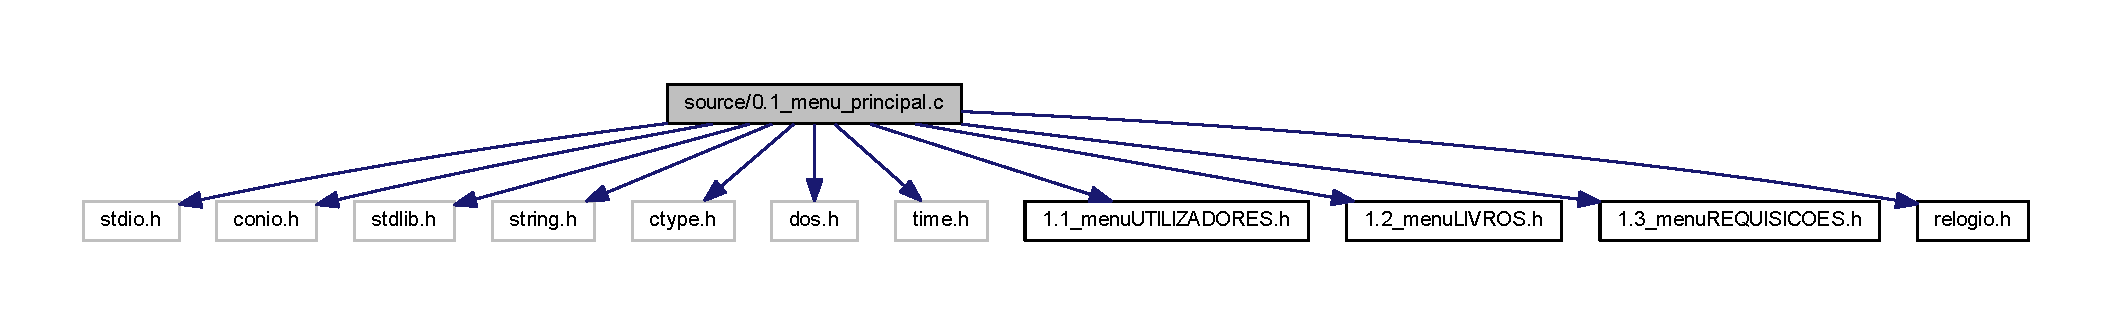
\includegraphics[width=350pt]{0_81__menu__principal_8c__incl}
\end{center}
\end{figure}
\subsection*{Macros}
\begin{DoxyCompactItemize}
\item 
\#define \hyperlink{0_81__menu__principal_8c_a56169c6a67c401a6efc300fb4ec07935}{R\+E\+T\+U\+R\+N\+T\+I\+M\+E}~15
\end{DoxyCompactItemize}
\subsection*{Functions}
\begin{DoxyCompactItemize}
\item 
void \hyperlink{0_81__menu__principal_8c_a575708342c73863481c539939d5bd21e}{limpa\+\_\+ecra} ()
\item 
void \hyperlink{0_81__menu__principal_8c_a1ec3fb130b1c938c318d10717fd48294}{M\+E\+N\+U\+\_\+\+P\+R\+I\+N\+C\+I\+P\+A\+L} ()
\item 
int \hyperlink{0_81__menu__principal_8c_ae66f6b31b5ad750f1fe042a706a4e3d4}{main} ()
\end{DoxyCompactItemize}


\subsection{Macro Definition Documentation}
\hypertarget{0_81__menu__principal_8c_a56169c6a67c401a6efc300fb4ec07935}{\index{0.\+1\+\_\+menu\+\_\+principal.\+c@{0.\+1\+\_\+menu\+\_\+principal.\+c}!R\+E\+T\+U\+R\+N\+T\+I\+M\+E@{R\+E\+T\+U\+R\+N\+T\+I\+M\+E}}
\index{R\+E\+T\+U\+R\+N\+T\+I\+M\+E@{R\+E\+T\+U\+R\+N\+T\+I\+M\+E}!0.\+1\+\_\+menu\+\_\+principal.\+c@{0.\+1\+\_\+menu\+\_\+principal.\+c}}
\subsubsection[{R\+E\+T\+U\+R\+N\+T\+I\+M\+E}]{\setlength{\rightskip}{0pt plus 5cm}\#define R\+E\+T\+U\+R\+N\+T\+I\+M\+E~15}}\label{0_81__menu__principal_8c_a56169c6a67c401a6efc300fb4ec07935}


\subsection{Function Documentation}
\hypertarget{0_81__menu__principal_8c_a575708342c73863481c539939d5bd21e}{\index{0.\+1\+\_\+menu\+\_\+principal.\+c@{0.\+1\+\_\+menu\+\_\+principal.\+c}!limpa\+\_\+ecra@{limpa\+\_\+ecra}}
\index{limpa\+\_\+ecra@{limpa\+\_\+ecra}!0.\+1\+\_\+menu\+\_\+principal.\+c@{0.\+1\+\_\+menu\+\_\+principal.\+c}}
\subsubsection[{limpa\+\_\+ecra}]{\setlength{\rightskip}{0pt plus 5cm}void limpa\+\_\+ecra (
\begin{DoxyParamCaption}
{}
\end{DoxyParamCaption}
)}}\label{0_81__menu__principal_8c_a575708342c73863481c539939d5bd21e}
Fun��o utilizada para limpar o ecr�. Assim, sempre que necess�rio, basta chamar \hyperlink{0_81__menu__principal_8c_a575708342c73863481c539939d5bd21e}{limpa\+\_\+ecra()} 

Here is the caller graph for this function\+:\nopagebreak
\begin{figure}[H]
\begin{center}
\leavevmode
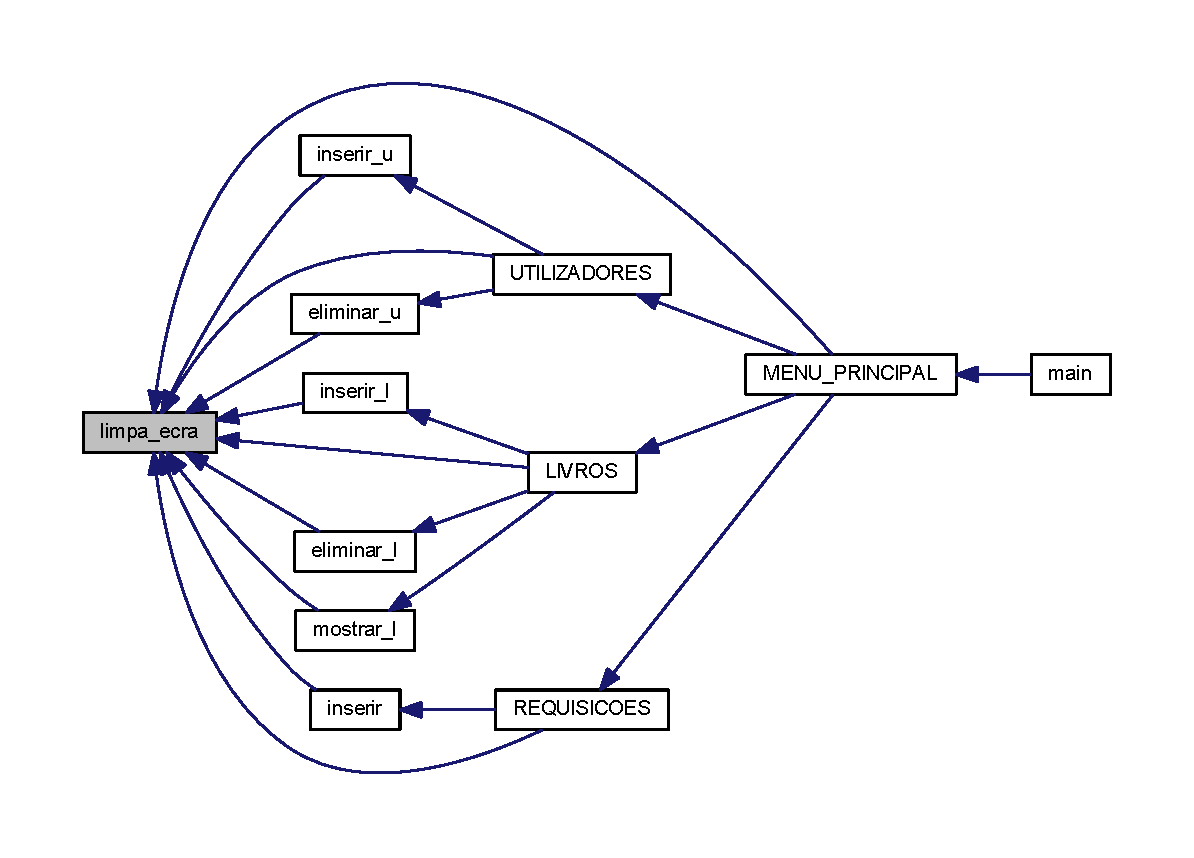
\includegraphics[width=350pt]{0_81__menu__principal_8c_a575708342c73863481c539939d5bd21e_icgraph}
\end{center}
\end{figure}


\hypertarget{0_81__menu__principal_8c_ae66f6b31b5ad750f1fe042a706a4e3d4}{\index{0.\+1\+\_\+menu\+\_\+principal.\+c@{0.\+1\+\_\+menu\+\_\+principal.\+c}!main@{main}}
\index{main@{main}!0.\+1\+\_\+menu\+\_\+principal.\+c@{0.\+1\+\_\+menu\+\_\+principal.\+c}}
\subsubsection[{main}]{\setlength{\rightskip}{0pt plus 5cm}int main (
\begin{DoxyParamCaption}
{}
\end{DoxyParamCaption}
)}}\label{0_81__menu__principal_8c_ae66f6b31b5ad750f1fe042a706a4e3d4}


Here is the call graph for this function\+:\nopagebreak
\begin{figure}[H]
\begin{center}
\leavevmode
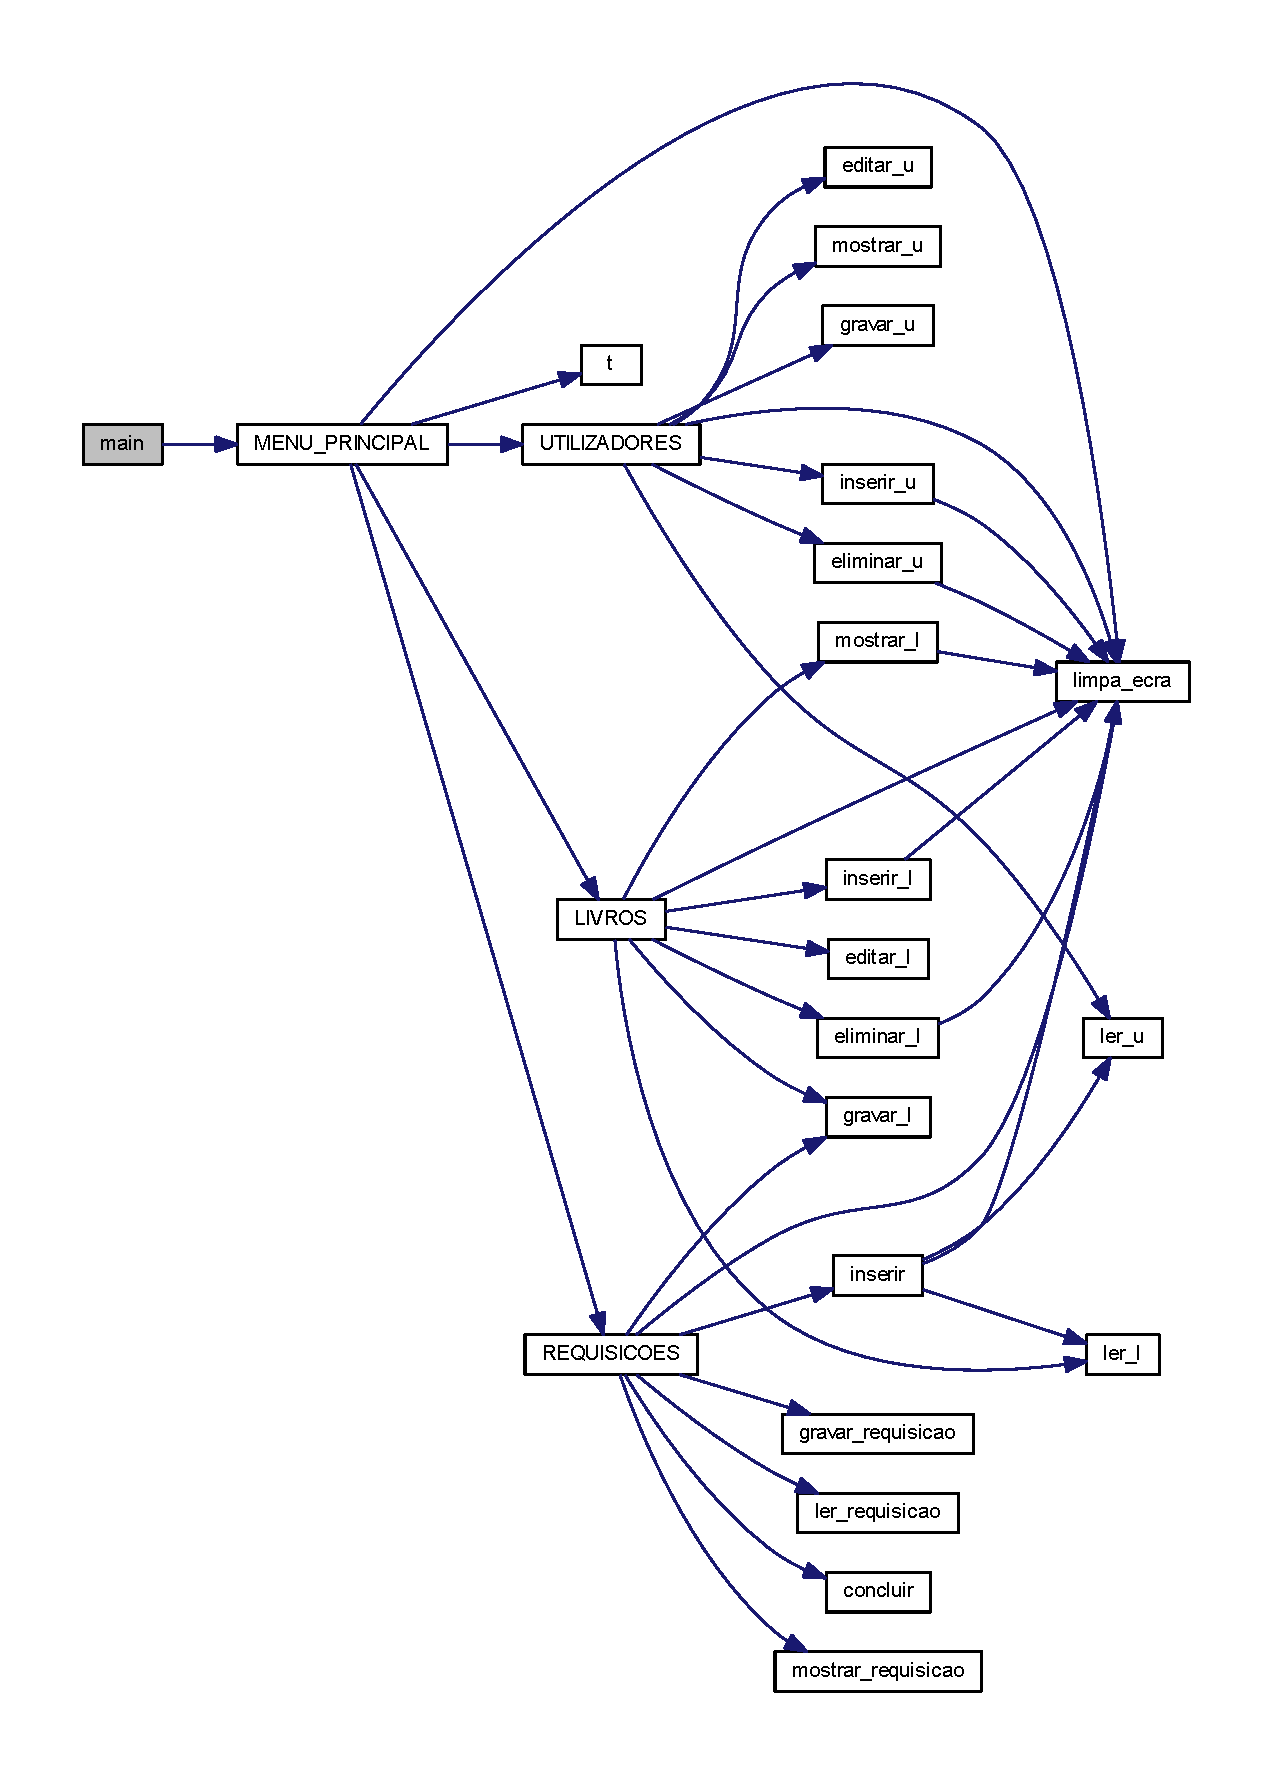
\includegraphics[width=350pt]{0_81__menu__principal_8c_ae66f6b31b5ad750f1fe042a706a4e3d4_cgraph}
\end{center}
\end{figure}


\hypertarget{0_81__menu__principal_8c_a1ec3fb130b1c938c318d10717fd48294}{\index{0.\+1\+\_\+menu\+\_\+principal.\+c@{0.\+1\+\_\+menu\+\_\+principal.\+c}!M\+E\+N\+U\+\_\+\+P\+R\+I\+N\+C\+I\+P\+A\+L@{M\+E\+N\+U\+\_\+\+P\+R\+I\+N\+C\+I\+P\+A\+L}}
\index{M\+E\+N\+U\+\_\+\+P\+R\+I\+N\+C\+I\+P\+A\+L@{M\+E\+N\+U\+\_\+\+P\+R\+I\+N\+C\+I\+P\+A\+L}!0.\+1\+\_\+menu\+\_\+principal.\+c@{0.\+1\+\_\+menu\+\_\+principal.\+c}}
\subsubsection[{M\+E\+N\+U\+\_\+\+P\+R\+I\+N\+C\+I\+P\+A\+L}]{\setlength{\rightskip}{0pt plus 5cm}void M\+E\+N\+U\+\_\+\+P\+R\+I\+N\+C\+I\+P\+A\+L (
\begin{DoxyParamCaption}
{}
\end{DoxyParamCaption}
)}}\label{0_81__menu__principal_8c_a1ec3fb130b1c938c318d10717fd48294}
Estrutura global do programa B\+I\+B\+L\+I\+O\+T\+E\+C\+A\+T\+I\+C 

Here is the call graph for this function\+:\nopagebreak
\begin{figure}[H]
\begin{center}
\leavevmode
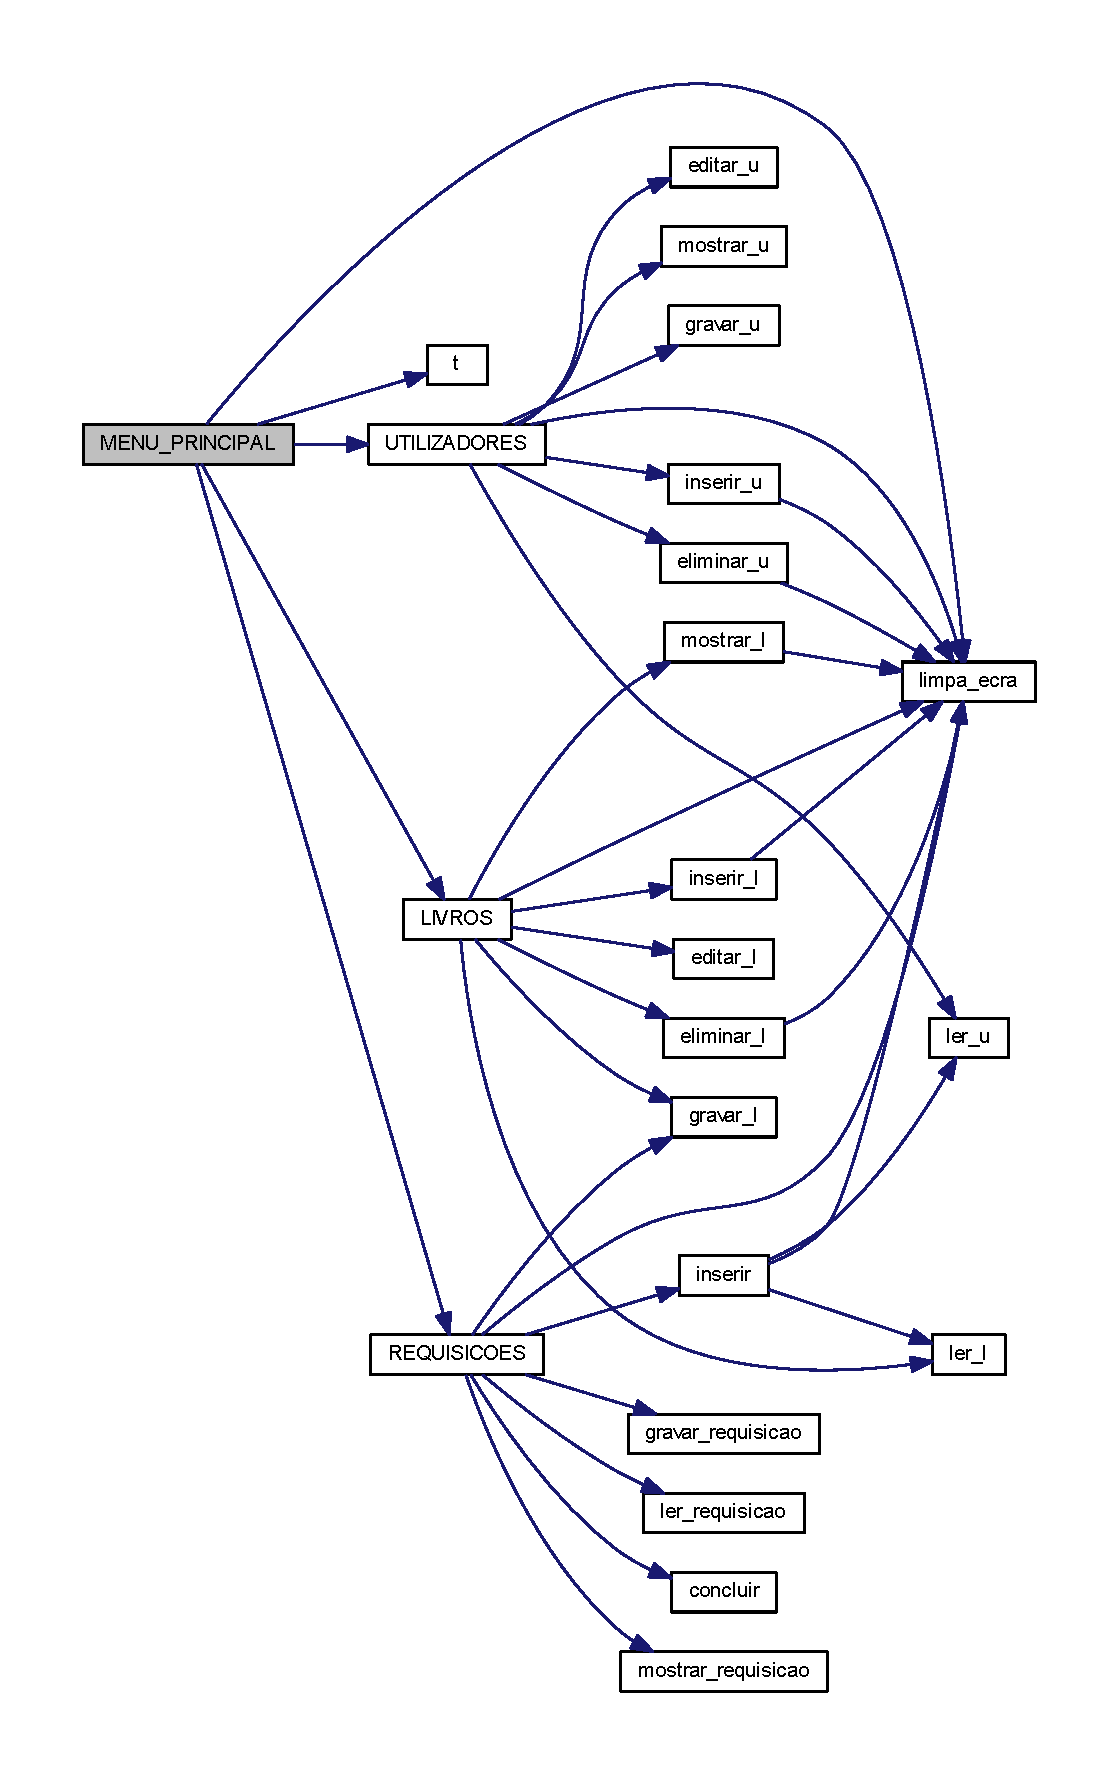
\includegraphics[height=550pt]{0_81__menu__principal_8c_a1ec3fb130b1c938c318d10717fd48294_cgraph}
\end{center}
\end{figure}




Here is the caller graph for this function\+:\nopagebreak
\begin{figure}[H]
\begin{center}
\leavevmode
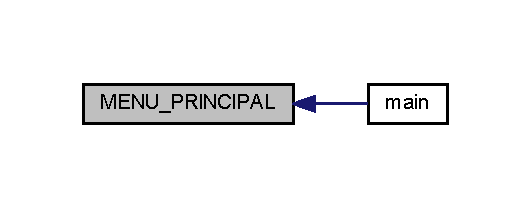
\includegraphics[width=255pt]{0_81__menu__principal_8c_a1ec3fb130b1c938c318d10717fd48294_icgraph}
\end{center}
\end{figure}



\hypertarget{1_81__menu_u_t_i_l_i_z_a_d_o_r_e_s_8h}{\section{source/1.1\+\_\+menu\+U\+T\+I\+L\+I\+Z\+A\+D\+O\+R\+E\+S.h File Reference}
\label{1_81__menu_u_t_i_l_i_z_a_d_o_r_e_s_8h}\index{source/1.\+1\+\_\+menu\+U\+T\+I\+L\+I\+Z\+A\+D\+O\+R\+E\+S.\+h@{source/1.\+1\+\_\+menu\+U\+T\+I\+L\+I\+Z\+A\+D\+O\+R\+E\+S.\+h}}
}
This graph shows which files directly or indirectly include this file\+:\nopagebreak
\begin{figure}[H]
\begin{center}
\leavevmode
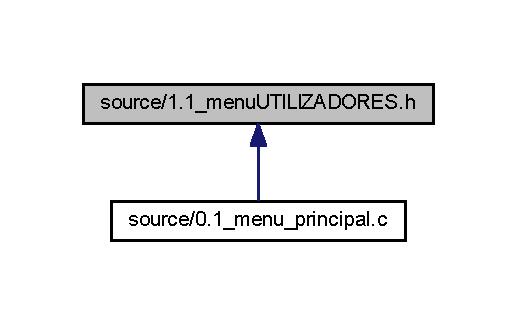
\includegraphics[width=248pt]{1_81__menu_u_t_i_l_i_z_a_d_o_r_e_s_8h__dep__incl}
\end{center}
\end{figure}
\subsection*{Data Structures}
\begin{DoxyCompactItemize}
\item 
struct \hyperlink{structutilizador}{utilizador}
\end{DoxyCompactItemize}
\subsection*{Macros}
\begin{DoxyCompactItemize}
\item 
\#define \hyperlink{1_81__menu_u_t_i_l_i_z_a_d_o_r_e_s_8h_af146485306ae74a2edf18636300fd107}{N\+R}~100
\end{DoxyCompactItemize}
\subsection*{Functions}
\begin{DoxyCompactItemize}
\item 
void \hyperlink{1_81__menu_u_t_i_l_i_z_a_d_o_r_e_s_8h_a0ec030ae5d28bb3d4afa78c75f244667}{ler\+\_\+u} (\hyperlink{structutilizador}{utilizador} $\ast$x)
\item 
void \hyperlink{1_81__menu_u_t_i_l_i_z_a_d_o_r_e_s_8h_aa717e0d2578028ffbf423f03a3942186}{gravar\+\_\+u} (\hyperlink{structutilizador}{utilizador} $\ast$x)
\item 
void \hyperlink{1_81__menu_u_t_i_l_i_z_a_d_o_r_e_s_8h_a5e68fd833522d40a62009b56c8f2c37f}{inserir\+\_\+u} (\hyperlink{structutilizador}{utilizador} $\ast$x)
\item 
int \hyperlink{1_81__menu_u_t_i_l_i_z_a_d_o_r_e_s_8h_a41f3d76f47e2459f90c909db59a958b5}{editar\+\_\+u} (\hyperlink{structutilizador}{utilizador} $\ast$x)
\item 
int \hyperlink{1_81__menu_u_t_i_l_i_z_a_d_o_r_e_s_8h_aa8434c82c844e4d6f4dceae0a9ec11b6}{eliminar\+\_\+u} (\hyperlink{structutilizador}{utilizador} $\ast$x)
\item 
void \hyperlink{1_81__menu_u_t_i_l_i_z_a_d_o_r_e_s_8h_a92ee6313ede592851e9f8756f184960f}{mostrar\+\_\+u} (\hyperlink{structutilizador}{utilizador} $\ast$x)
\item 
void \hyperlink{1_81__menu_u_t_i_l_i_z_a_d_o_r_e_s_8h_a10969cc094da713694ed847af267c9c0}{U\+T\+I\+L\+I\+Z\+A\+D\+O\+R\+E\+S} (void)
\end{DoxyCompactItemize}


\subsection{Macro Definition Documentation}
\hypertarget{1_81__menu_u_t_i_l_i_z_a_d_o_r_e_s_8h_af146485306ae74a2edf18636300fd107}{\index{1.\+1\+\_\+menu\+U\+T\+I\+L\+I\+Z\+A\+D\+O\+R\+E\+S.\+h@{1.\+1\+\_\+menu\+U\+T\+I\+L\+I\+Z\+A\+D\+O\+R\+E\+S.\+h}!N\+R@{N\+R}}
\index{N\+R@{N\+R}!1.\+1\+\_\+menu\+U\+T\+I\+L\+I\+Z\+A\+D\+O\+R\+E\+S.\+h@{1.\+1\+\_\+menu\+U\+T\+I\+L\+I\+Z\+A\+D\+O\+R\+E\+S.\+h}}
\subsubsection[{N\+R}]{\setlength{\rightskip}{0pt plus 5cm}\#define N\+R~100}}\label{1_81__menu_u_t_i_l_i_z_a_d_o_r_e_s_8h_af146485306ae74a2edf18636300fd107}


\subsection{Function Documentation}
\hypertarget{1_81__menu_u_t_i_l_i_z_a_d_o_r_e_s_8h_a41f3d76f47e2459f90c909db59a958b5}{\index{1.\+1\+\_\+menu\+U\+T\+I\+L\+I\+Z\+A\+D\+O\+R\+E\+S.\+h@{1.\+1\+\_\+menu\+U\+T\+I\+L\+I\+Z\+A\+D\+O\+R\+E\+S.\+h}!editar\+\_\+u@{editar\+\_\+u}}
\index{editar\+\_\+u@{editar\+\_\+u}!1.\+1\+\_\+menu\+U\+T\+I\+L\+I\+Z\+A\+D\+O\+R\+E\+S.\+h@{1.\+1\+\_\+menu\+U\+T\+I\+L\+I\+Z\+A\+D\+O\+R\+E\+S.\+h}}
\subsubsection[{editar\+\_\+u}]{\setlength{\rightskip}{0pt plus 5cm}int editar\+\_\+u (
\begin{DoxyParamCaption}
\item[{{\bf utilizador} $\ast$}]{x}
\end{DoxyParamCaption}
)}}\label{1_81__menu_u_t_i_l_i_z_a_d_o_r_e_s_8h_a41f3d76f47e2459f90c909db59a958b5}
O programa verifica se o I\+D de utilizador existe e, se sim, procese �s edi��es das informa��es.

S\+Ee o utilizador estava eliminado, e possivel editado e ele volta ao estado 1, significando que volta a estar disponivel 

Here is the caller graph for this function\+:\nopagebreak
\begin{figure}[H]
\begin{center}
\leavevmode
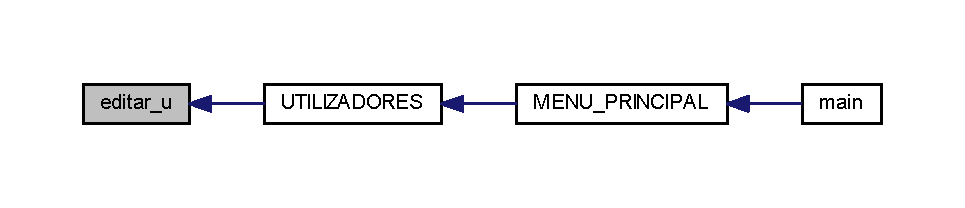
\includegraphics[width=350pt]{1_81__menu_u_t_i_l_i_z_a_d_o_r_e_s_8h_a41f3d76f47e2459f90c909db59a958b5_icgraph}
\end{center}
\end{figure}


\hypertarget{1_81__menu_u_t_i_l_i_z_a_d_o_r_e_s_8h_aa8434c82c844e4d6f4dceae0a9ec11b6}{\index{1.\+1\+\_\+menu\+U\+T\+I\+L\+I\+Z\+A\+D\+O\+R\+E\+S.\+h@{1.\+1\+\_\+menu\+U\+T\+I\+L\+I\+Z\+A\+D\+O\+R\+E\+S.\+h}!eliminar\+\_\+u@{eliminar\+\_\+u}}
\index{eliminar\+\_\+u@{eliminar\+\_\+u}!1.\+1\+\_\+menu\+U\+T\+I\+L\+I\+Z\+A\+D\+O\+R\+E\+S.\+h@{1.\+1\+\_\+menu\+U\+T\+I\+L\+I\+Z\+A\+D\+O\+R\+E\+S.\+h}}
\subsubsection[{eliminar\+\_\+u}]{\setlength{\rightskip}{0pt plus 5cm}int eliminar\+\_\+u (
\begin{DoxyParamCaption}
\item[{{\bf utilizador} $\ast$}]{x}
\end{DoxyParamCaption}
)}}\label{1_81__menu_u_t_i_l_i_z_a_d_o_r_e_s_8h_aa8434c82c844e4d6f4dceae0a9ec11b6}
verifica de o I\+D de utilizador existe

Procura pelos utilizadores existentes, pois se o estado estiver a 2 significa que ja se encontra eliminado.

Se nao estiver eliminado, altera entao o estado para 2. 

Here is the call graph for this function\+:\nopagebreak
\begin{figure}[H]
\begin{center}
\leavevmode
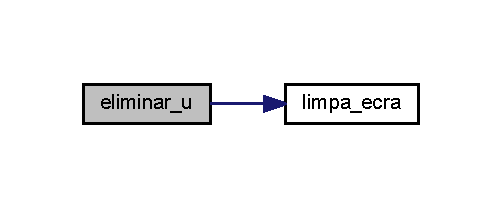
\includegraphics[width=241pt]{1_81__menu_u_t_i_l_i_z_a_d_o_r_e_s_8h_aa8434c82c844e4d6f4dceae0a9ec11b6_cgraph}
\end{center}
\end{figure}




Here is the caller graph for this function\+:\nopagebreak
\begin{figure}[H]
\begin{center}
\leavevmode
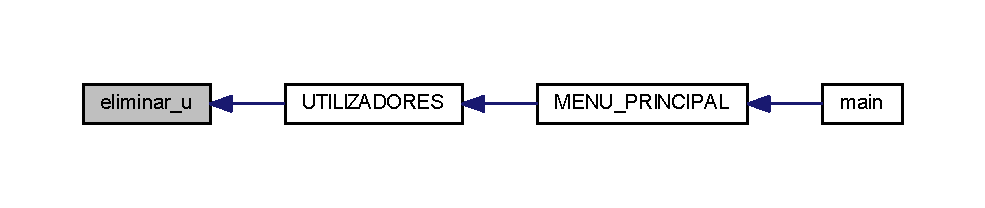
\includegraphics[width=350pt]{1_81__menu_u_t_i_l_i_z_a_d_o_r_e_s_8h_aa8434c82c844e4d6f4dceae0a9ec11b6_icgraph}
\end{center}
\end{figure}


\hypertarget{1_81__menu_u_t_i_l_i_z_a_d_o_r_e_s_8h_aa717e0d2578028ffbf423f03a3942186}{\index{1.\+1\+\_\+menu\+U\+T\+I\+L\+I\+Z\+A\+D\+O\+R\+E\+S.\+h@{1.\+1\+\_\+menu\+U\+T\+I\+L\+I\+Z\+A\+D\+O\+R\+E\+S.\+h}!gravar\+\_\+u@{gravar\+\_\+u}}
\index{gravar\+\_\+u@{gravar\+\_\+u}!1.\+1\+\_\+menu\+U\+T\+I\+L\+I\+Z\+A\+D\+O\+R\+E\+S.\+h@{1.\+1\+\_\+menu\+U\+T\+I\+L\+I\+Z\+A\+D\+O\+R\+E\+S.\+h}}
\subsubsection[{gravar\+\_\+u}]{\setlength{\rightskip}{0pt plus 5cm}void gravar\+\_\+u (
\begin{DoxyParamCaption}
\item[{{\bf utilizador} $\ast$}]{x}
\end{DoxyParamCaption}
)}}\label{1_81__menu_u_t_i_l_i_z_a_d_o_r_e_s_8h_aa717e0d2578028ffbf423f03a3942186}
Para abrir o programa e utilizado \char`\"{}wt\char`\"{}\+: w-\/ para escrever no ficheiro, t-\/ ficheiro de texto

O programa grava apenas utilizadores com estado diferente de 0, pois caso tal aconteca, os utilizadores nao existem 

Here is the caller graph for this function\+:\nopagebreak
\begin{figure}[H]
\begin{center}
\leavevmode
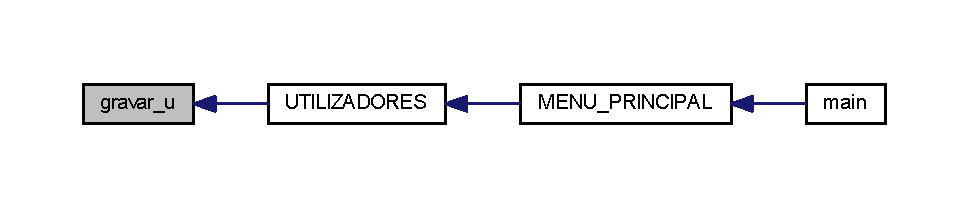
\includegraphics[width=350pt]{1_81__menu_u_t_i_l_i_z_a_d_o_r_e_s_8h_aa717e0d2578028ffbf423f03a3942186_icgraph}
\end{center}
\end{figure}


\hypertarget{1_81__menu_u_t_i_l_i_z_a_d_o_r_e_s_8h_a5e68fd833522d40a62009b56c8f2c37f}{\index{1.\+1\+\_\+menu\+U\+T\+I\+L\+I\+Z\+A\+D\+O\+R\+E\+S.\+h@{1.\+1\+\_\+menu\+U\+T\+I\+L\+I\+Z\+A\+D\+O\+R\+E\+S.\+h}!inserir\+\_\+u@{inserir\+\_\+u}}
\index{inserir\+\_\+u@{inserir\+\_\+u}!1.\+1\+\_\+menu\+U\+T\+I\+L\+I\+Z\+A\+D\+O\+R\+E\+S.\+h@{1.\+1\+\_\+menu\+U\+T\+I\+L\+I\+Z\+A\+D\+O\+R\+E\+S.\+h}}
\subsubsection[{inserir\+\_\+u}]{\setlength{\rightskip}{0pt plus 5cm}void inserir\+\_\+u (
\begin{DoxyParamCaption}
\item[{{\bf utilizador} $\ast$}]{x}
\end{DoxyParamCaption}
)}}\label{1_81__menu_u_t_i_l_i_z_a_d_o_r_e_s_8h_a5e68fd833522d40a62009b56c8f2c37f}
Se o utilizador nao pretender inserir um novo utilizador, basta inserir 0 para voltar.

� feita uma funcao que faz a atribuicao automatica dos I\+D's de utilizador.

Verifica se o I\+D inicial se encontra disponivel verificando o seu estado, se nao estiver, \char`\"{}avan�a mais um numero\char`\"{} at� que encontre um disponivel

Apos receber as informa��es, o programa coloca o estado de novos utilizadores a 1 (existente) 

Here is the call graph for this function\+:\nopagebreak
\begin{figure}[H]
\begin{center}
\leavevmode
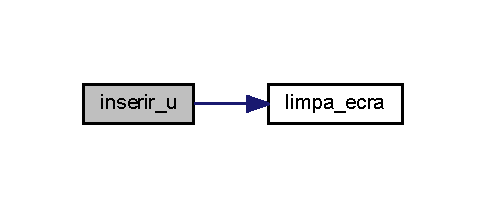
\includegraphics[width=233pt]{1_81__menu_u_t_i_l_i_z_a_d_o_r_e_s_8h_a5e68fd833522d40a62009b56c8f2c37f_cgraph}
\end{center}
\end{figure}




Here is the caller graph for this function\+:\nopagebreak
\begin{figure}[H]
\begin{center}
\leavevmode
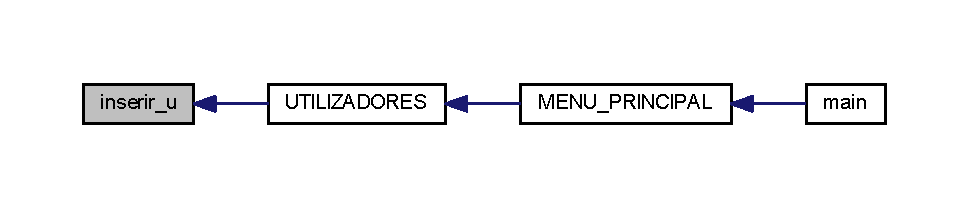
\includegraphics[width=350pt]{1_81__menu_u_t_i_l_i_z_a_d_o_r_e_s_8h_a5e68fd833522d40a62009b56c8f2c37f_icgraph}
\end{center}
\end{figure}


\hypertarget{1_81__menu_u_t_i_l_i_z_a_d_o_r_e_s_8h_a0ec030ae5d28bb3d4afa78c75f244667}{\index{1.\+1\+\_\+menu\+U\+T\+I\+L\+I\+Z\+A\+D\+O\+R\+E\+S.\+h@{1.\+1\+\_\+menu\+U\+T\+I\+L\+I\+Z\+A\+D\+O\+R\+E\+S.\+h}!ler\+\_\+u@{ler\+\_\+u}}
\index{ler\+\_\+u@{ler\+\_\+u}!1.\+1\+\_\+menu\+U\+T\+I\+L\+I\+Z\+A\+D\+O\+R\+E\+S.\+h@{1.\+1\+\_\+menu\+U\+T\+I\+L\+I\+Z\+A\+D\+O\+R\+E\+S.\+h}}
\subsubsection[{ler\+\_\+u}]{\setlength{\rightskip}{0pt plus 5cm}void ler\+\_\+u (
\begin{DoxyParamCaption}
\item[{{\bf utilizador} $\ast$}]{x}
\end{DoxyParamCaption}
)}}\label{1_81__menu_u_t_i_l_i_z_a_d_o_r_e_s_8h_a0ec030ae5d28bb3d4afa78c75f244667}
Para abrir o ficheiro � utilizado \char`\"{}rt\char`\"{}, que significa r-\/read e t-\/ficheiro de texto

O programa efetua a leitura no ficheito utilizadores.\+txt e l� as informa��es de I\+D's

de utilizadores que existam.

Se o estado de algum utilizador for igual a 0 o programa nao o le, pois significa que nao existe 

Here is the caller graph for this function\+:\nopagebreak
\begin{figure}[H]
\begin{center}
\leavevmode
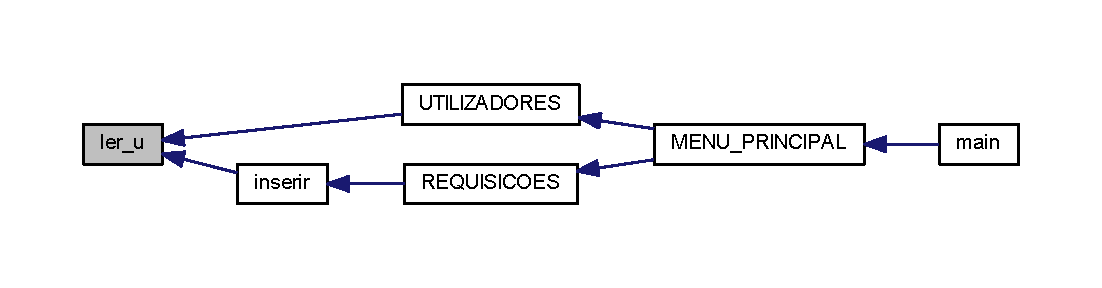
\includegraphics[width=350pt]{1_81__menu_u_t_i_l_i_z_a_d_o_r_e_s_8h_a0ec030ae5d28bb3d4afa78c75f244667_icgraph}
\end{center}
\end{figure}


\hypertarget{1_81__menu_u_t_i_l_i_z_a_d_o_r_e_s_8h_a92ee6313ede592851e9f8756f184960f}{\index{1.\+1\+\_\+menu\+U\+T\+I\+L\+I\+Z\+A\+D\+O\+R\+E\+S.\+h@{1.\+1\+\_\+menu\+U\+T\+I\+L\+I\+Z\+A\+D\+O\+R\+E\+S.\+h}!mostrar\+\_\+u@{mostrar\+\_\+u}}
\index{mostrar\+\_\+u@{mostrar\+\_\+u}!1.\+1\+\_\+menu\+U\+T\+I\+L\+I\+Z\+A\+D\+O\+R\+E\+S.\+h@{1.\+1\+\_\+menu\+U\+T\+I\+L\+I\+Z\+A\+D\+O\+R\+E\+S.\+h}}
\subsubsection[{mostrar\+\_\+u}]{\setlength{\rightskip}{0pt plus 5cm}void mostrar\+\_\+u (
\begin{DoxyParamCaption}
\item[{{\bf utilizador} $\ast$}]{x}
\end{DoxyParamCaption}
)}}\label{1_81__menu_u_t_i_l_i_z_a_d_o_r_e_s_8h_a92ee6313ede592851e9f8756f184960f}
Mostrar utilizadores com estado a 1

Se existirem utilizadores com estado=2, significa que estao eliminados e, como tal, mostra no fim a mensagem \char`\"{}eliminado\char`\"{} . Estes sao apenas mostrados no fim da lista. 

Here is the caller graph for this function\+:\nopagebreak
\begin{figure}[H]
\begin{center}
\leavevmode
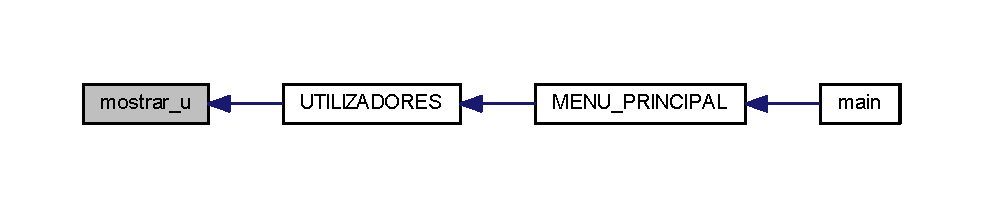
\includegraphics[width=350pt]{1_81__menu_u_t_i_l_i_z_a_d_o_r_e_s_8h_a92ee6313ede592851e9f8756f184960f_icgraph}
\end{center}
\end{figure}


\hypertarget{1_81__menu_u_t_i_l_i_z_a_d_o_r_e_s_8h_a10969cc094da713694ed847af267c9c0}{\index{1.\+1\+\_\+menu\+U\+T\+I\+L\+I\+Z\+A\+D\+O\+R\+E\+S.\+h@{1.\+1\+\_\+menu\+U\+T\+I\+L\+I\+Z\+A\+D\+O\+R\+E\+S.\+h}!U\+T\+I\+L\+I\+Z\+A\+D\+O\+R\+E\+S@{U\+T\+I\+L\+I\+Z\+A\+D\+O\+R\+E\+S}}
\index{U\+T\+I\+L\+I\+Z\+A\+D\+O\+R\+E\+S@{U\+T\+I\+L\+I\+Z\+A\+D\+O\+R\+E\+S}!1.\+1\+\_\+menu\+U\+T\+I\+L\+I\+Z\+A\+D\+O\+R\+E\+S.\+h@{1.\+1\+\_\+menu\+U\+T\+I\+L\+I\+Z\+A\+D\+O\+R\+E\+S.\+h}}
\subsubsection[{U\+T\+I\+L\+I\+Z\+A\+D\+O\+R\+E\+S}]{\setlength{\rightskip}{0pt plus 5cm}void U\+T\+I\+L\+I\+Z\+A\+D\+O\+R\+E\+S (
\begin{DoxyParamCaption}
\item[{void}]{}
\end{DoxyParamCaption}
)}}\label{1_81__menu_u_t_i_l_i_z_a_d_o_r_e_s_8h_a10969cc094da713694ed847af267c9c0}
id's iniciais de utilizadores apresentam estado igual a 0, quando forem utilizados passam a 1 

Here is the call graph for this function\+:\nopagebreak
\begin{figure}[H]
\begin{center}
\leavevmode
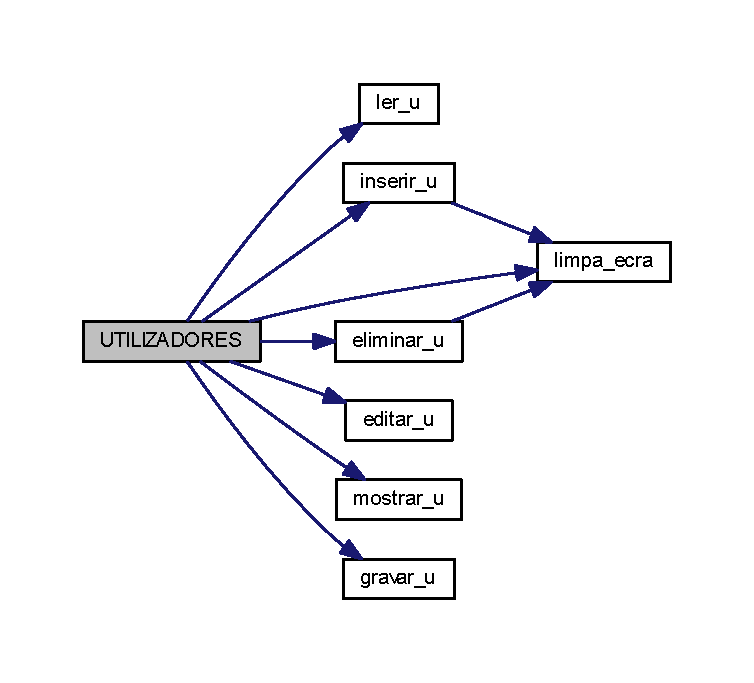
\includegraphics[width=350pt]{1_81__menu_u_t_i_l_i_z_a_d_o_r_e_s_8h_a10969cc094da713694ed847af267c9c0_cgraph}
\end{center}
\end{figure}




Here is the caller graph for this function\+:\nopagebreak
\begin{figure}[H]
\begin{center}
\leavevmode
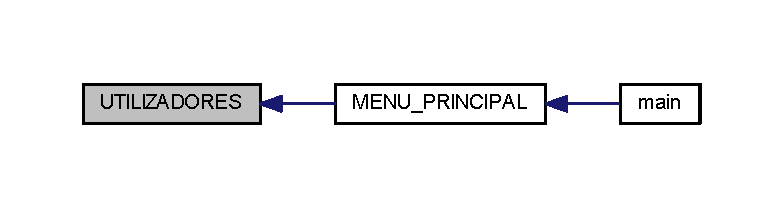
\includegraphics[width=350pt]{1_81__menu_u_t_i_l_i_z_a_d_o_r_e_s_8h_a10969cc094da713694ed847af267c9c0_icgraph}
\end{center}
\end{figure}



\hypertarget{1_82__menu_l_i_v_r_o_s_8h}{\section{source/1.2\+\_\+menu\+L\+I\+V\+R\+O\+S.h File Reference}
\label{1_82__menu_l_i_v_r_o_s_8h}\index{source/1.\+2\+\_\+menu\+L\+I\+V\+R\+O\+S.\+h@{source/1.\+2\+\_\+menu\+L\+I\+V\+R\+O\+S.\+h}}
}
This graph shows which files directly or indirectly include this file\+:\nopagebreak
\begin{figure}[H]
\begin{center}
\leavevmode
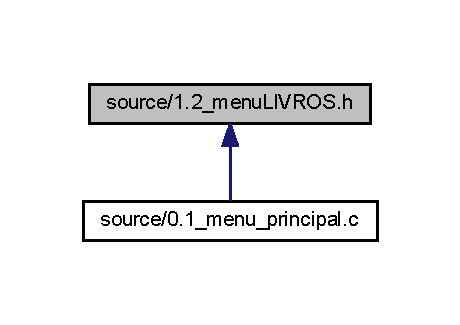
\includegraphics[width=221pt]{1_82__menu_l_i_v_r_o_s_8h__dep__incl}
\end{center}
\end{figure}
\subsection*{Data Structures}
\begin{DoxyCompactItemize}
\item 
struct \hyperlink{structlivro}{livro}
\end{DoxyCompactItemize}
\subsection*{Macros}
\begin{DoxyCompactItemize}
\item 
\#define \hyperlink{1_82__menu_l_i_v_r_o_s_8h_a52037c938e3c1b126c6277da5ca689d0}{M}~100
\end{DoxyCompactItemize}
\subsection*{Functions}
\begin{DoxyCompactItemize}
\item 
void \hyperlink{1_82__menu_l_i_v_r_o_s_8h_aec15f06157938329587cc93e4fb812ab}{ler\+\_\+l} (\hyperlink{structlivro}{livro} $\ast$y)
\item 
void \hyperlink{1_82__menu_l_i_v_r_o_s_8h_a1c91cb4dfb1278efa275317e94b76790}{gravar\+\_\+l} (\hyperlink{structlivro}{livro} $\ast$y)
\item 
void \hyperlink{1_82__menu_l_i_v_r_o_s_8h_a11485b72bfb78f02f72edab1d00cb0d5}{inserir\+\_\+l} (\hyperlink{structlivro}{livro} $\ast$y)
\item 
int \hyperlink{1_82__menu_l_i_v_r_o_s_8h_acd34e57b816a8b1b99d4aad0510c72a3}{editar\+\_\+l} (\hyperlink{structlivro}{livro} $\ast$y)
\item 
int \hyperlink{1_82__menu_l_i_v_r_o_s_8h_af8eb970526c202f594da1c16355fa43a}{eliminar\+\_\+l} (\hyperlink{structlivro}{livro} $\ast$y)
\item 
void \hyperlink{1_82__menu_l_i_v_r_o_s_8h_a41a1c98261117fbe5e6f0ebbcec5f9ac}{mostrar\+\_\+l} (\hyperlink{structlivro}{livro} $\ast$y)
\item 
void \hyperlink{1_82__menu_l_i_v_r_o_s_8h_a4e85258e55525e765829f28c4911eb9e}{L\+I\+V\+R\+O\+S} (void)
\end{DoxyCompactItemize}


\subsection{Macro Definition Documentation}
\hypertarget{1_82__menu_l_i_v_r_o_s_8h_a52037c938e3c1b126c6277da5ca689d0}{\index{1.\+2\+\_\+menu\+L\+I\+V\+R\+O\+S.\+h@{1.\+2\+\_\+menu\+L\+I\+V\+R\+O\+S.\+h}!M@{M}}
\index{M@{M}!1.\+2\+\_\+menu\+L\+I\+V\+R\+O\+S.\+h@{1.\+2\+\_\+menu\+L\+I\+V\+R\+O\+S.\+h}}
\subsubsection[{M}]{\setlength{\rightskip}{0pt plus 5cm}\#define M~100}}\label{1_82__menu_l_i_v_r_o_s_8h_a52037c938e3c1b126c6277da5ca689d0}


\subsection{Function Documentation}
\hypertarget{1_82__menu_l_i_v_r_o_s_8h_acd34e57b816a8b1b99d4aad0510c72a3}{\index{1.\+2\+\_\+menu\+L\+I\+V\+R\+O\+S.\+h@{1.\+2\+\_\+menu\+L\+I\+V\+R\+O\+S.\+h}!editar\+\_\+l@{editar\+\_\+l}}
\index{editar\+\_\+l@{editar\+\_\+l}!1.\+2\+\_\+menu\+L\+I\+V\+R\+O\+S.\+h@{1.\+2\+\_\+menu\+L\+I\+V\+R\+O\+S.\+h}}
\subsubsection[{editar\+\_\+l}]{\setlength{\rightskip}{0pt plus 5cm}int editar\+\_\+l (
\begin{DoxyParamCaption}
\item[{{\bf livro} $\ast$}]{y}
\end{DoxyParamCaption}
)}}\label{1_82__menu_l_i_v_r_o_s_8h_acd34e57b816a8b1b99d4aad0510c72a3}


Here is the caller graph for this function\+:\nopagebreak
\begin{figure}[H]
\begin{center}
\leavevmode
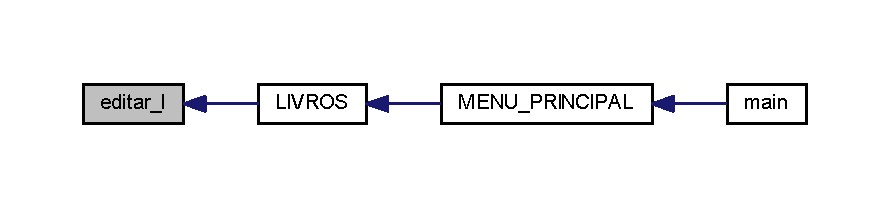
\includegraphics[width=350pt]{1_82__menu_l_i_v_r_o_s_8h_acd34e57b816a8b1b99d4aad0510c72a3_icgraph}
\end{center}
\end{figure}


\hypertarget{1_82__menu_l_i_v_r_o_s_8h_af8eb970526c202f594da1c16355fa43a}{\index{1.\+2\+\_\+menu\+L\+I\+V\+R\+O\+S.\+h@{1.\+2\+\_\+menu\+L\+I\+V\+R\+O\+S.\+h}!eliminar\+\_\+l@{eliminar\+\_\+l}}
\index{eliminar\+\_\+l@{eliminar\+\_\+l}!1.\+2\+\_\+menu\+L\+I\+V\+R\+O\+S.\+h@{1.\+2\+\_\+menu\+L\+I\+V\+R\+O\+S.\+h}}
\subsubsection[{eliminar\+\_\+l}]{\setlength{\rightskip}{0pt plus 5cm}int eliminar\+\_\+l (
\begin{DoxyParamCaption}
\item[{{\bf livro} $\ast$}]{y}
\end{DoxyParamCaption}
)}}\label{1_82__menu_l_i_v_r_o_s_8h_af8eb970526c202f594da1c16355fa43a}


Here is the call graph for this function\+:\nopagebreak
\begin{figure}[H]
\begin{center}
\leavevmode
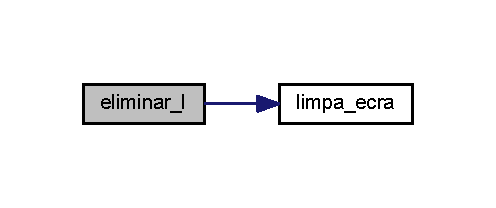
\includegraphics[width=238pt]{1_82__menu_l_i_v_r_o_s_8h_af8eb970526c202f594da1c16355fa43a_cgraph}
\end{center}
\end{figure}




Here is the caller graph for this function\+:\nopagebreak
\begin{figure}[H]
\begin{center}
\leavevmode
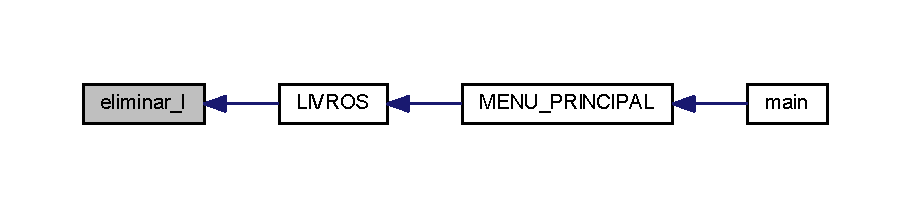
\includegraphics[width=350pt]{1_82__menu_l_i_v_r_o_s_8h_af8eb970526c202f594da1c16355fa43a_icgraph}
\end{center}
\end{figure}


\hypertarget{1_82__menu_l_i_v_r_o_s_8h_a1c91cb4dfb1278efa275317e94b76790}{\index{1.\+2\+\_\+menu\+L\+I\+V\+R\+O\+S.\+h@{1.\+2\+\_\+menu\+L\+I\+V\+R\+O\+S.\+h}!gravar\+\_\+l@{gravar\+\_\+l}}
\index{gravar\+\_\+l@{gravar\+\_\+l}!1.\+2\+\_\+menu\+L\+I\+V\+R\+O\+S.\+h@{1.\+2\+\_\+menu\+L\+I\+V\+R\+O\+S.\+h}}
\subsubsection[{gravar\+\_\+l}]{\setlength{\rightskip}{0pt plus 5cm}void gravar\+\_\+l (
\begin{DoxyParamCaption}
\item[{{\bf livro} $\ast$}]{y}
\end{DoxyParamCaption}
)}}\label{1_82__menu_l_i_v_r_o_s_8h_a1c91cb4dfb1278efa275317e94b76790}


Here is the caller graph for this function\+:\nopagebreak
\begin{figure}[H]
\begin{center}
\leavevmode
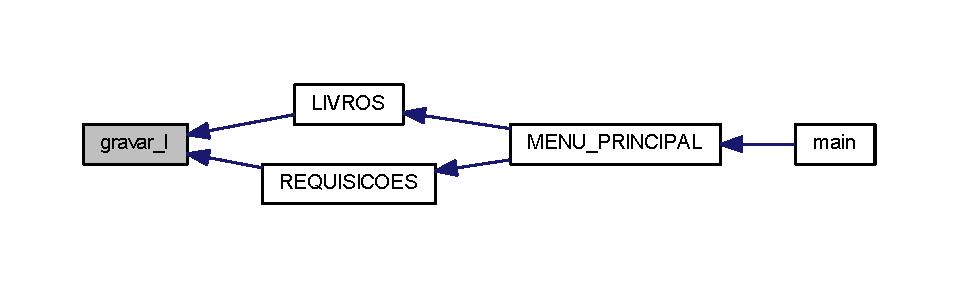
\includegraphics[width=350pt]{1_82__menu_l_i_v_r_o_s_8h_a1c91cb4dfb1278efa275317e94b76790_icgraph}
\end{center}
\end{figure}


\hypertarget{1_82__menu_l_i_v_r_o_s_8h_a11485b72bfb78f02f72edab1d00cb0d5}{\index{1.\+2\+\_\+menu\+L\+I\+V\+R\+O\+S.\+h@{1.\+2\+\_\+menu\+L\+I\+V\+R\+O\+S.\+h}!inserir\+\_\+l@{inserir\+\_\+l}}
\index{inserir\+\_\+l@{inserir\+\_\+l}!1.\+2\+\_\+menu\+L\+I\+V\+R\+O\+S.\+h@{1.\+2\+\_\+menu\+L\+I\+V\+R\+O\+S.\+h}}
\subsubsection[{inserir\+\_\+l}]{\setlength{\rightskip}{0pt plus 5cm}void inserir\+\_\+l (
\begin{DoxyParamCaption}
\item[{{\bf livro} $\ast$}]{y}
\end{DoxyParamCaption}
)}}\label{1_82__menu_l_i_v_r_o_s_8h_a11485b72bfb78f02f72edab1d00cb0d5}


Here is the call graph for this function\+:\nopagebreak
\begin{figure}[H]
\begin{center}
\leavevmode
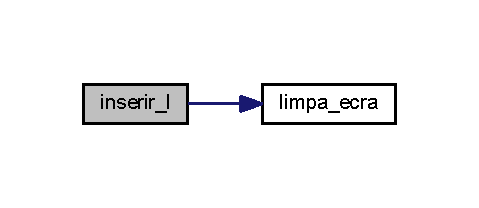
\includegraphics[width=230pt]{1_82__menu_l_i_v_r_o_s_8h_a11485b72bfb78f02f72edab1d00cb0d5_cgraph}
\end{center}
\end{figure}




Here is the caller graph for this function\+:\nopagebreak
\begin{figure}[H]
\begin{center}
\leavevmode
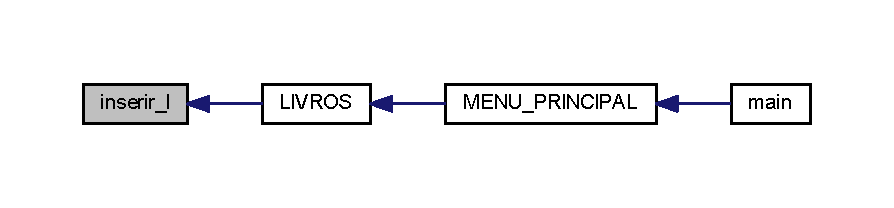
\includegraphics[width=350pt]{1_82__menu_l_i_v_r_o_s_8h_a11485b72bfb78f02f72edab1d00cb0d5_icgraph}
\end{center}
\end{figure}


\hypertarget{1_82__menu_l_i_v_r_o_s_8h_aec15f06157938329587cc93e4fb812ab}{\index{1.\+2\+\_\+menu\+L\+I\+V\+R\+O\+S.\+h@{1.\+2\+\_\+menu\+L\+I\+V\+R\+O\+S.\+h}!ler\+\_\+l@{ler\+\_\+l}}
\index{ler\+\_\+l@{ler\+\_\+l}!1.\+2\+\_\+menu\+L\+I\+V\+R\+O\+S.\+h@{1.\+2\+\_\+menu\+L\+I\+V\+R\+O\+S.\+h}}
\subsubsection[{ler\+\_\+l}]{\setlength{\rightskip}{0pt plus 5cm}void ler\+\_\+l (
\begin{DoxyParamCaption}
\item[{{\bf livro} $\ast$}]{y}
\end{DoxyParamCaption}
)}}\label{1_82__menu_l_i_v_r_o_s_8h_aec15f06157938329587cc93e4fb812ab}


Here is the caller graph for this function\+:\nopagebreak
\begin{figure}[H]
\begin{center}
\leavevmode
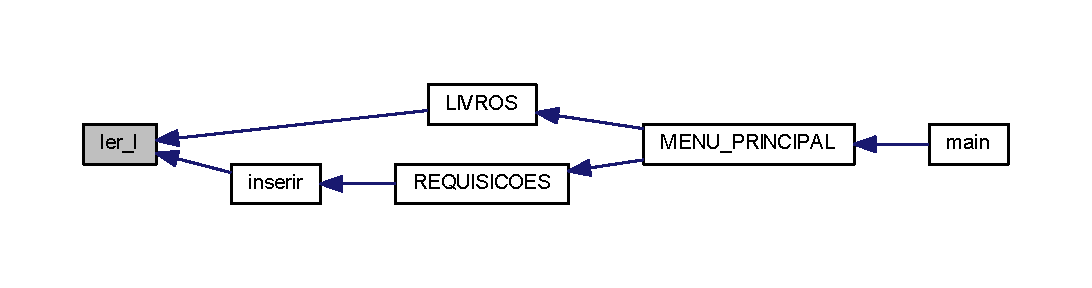
\includegraphics[width=350pt]{1_82__menu_l_i_v_r_o_s_8h_aec15f06157938329587cc93e4fb812ab_icgraph}
\end{center}
\end{figure}


\hypertarget{1_82__menu_l_i_v_r_o_s_8h_a4e85258e55525e765829f28c4911eb9e}{\index{1.\+2\+\_\+menu\+L\+I\+V\+R\+O\+S.\+h@{1.\+2\+\_\+menu\+L\+I\+V\+R\+O\+S.\+h}!L\+I\+V\+R\+O\+S@{L\+I\+V\+R\+O\+S}}
\index{L\+I\+V\+R\+O\+S@{L\+I\+V\+R\+O\+S}!1.\+2\+\_\+menu\+L\+I\+V\+R\+O\+S.\+h@{1.\+2\+\_\+menu\+L\+I\+V\+R\+O\+S.\+h}}
\subsubsection[{L\+I\+V\+R\+O\+S}]{\setlength{\rightskip}{0pt plus 5cm}void {\bf L\+I\+V\+R\+O\+S} (
\begin{DoxyParamCaption}
\item[{void}]{}
\end{DoxyParamCaption}
)}}\label{1_82__menu_l_i_v_r_o_s_8h_a4e85258e55525e765829f28c4911eb9e}


Here is the call graph for this function\+:\nopagebreak
\begin{figure}[H]
\begin{center}
\leavevmode
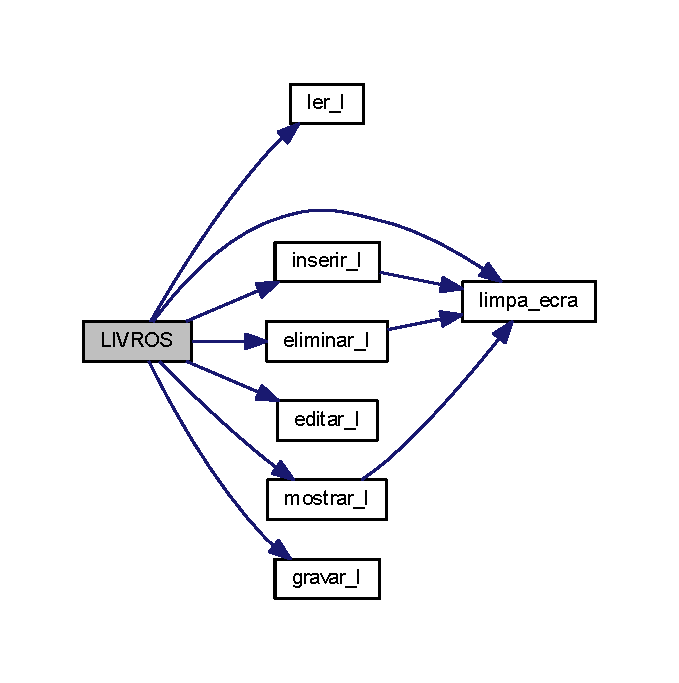
\includegraphics[width=326pt]{1_82__menu_l_i_v_r_o_s_8h_a4e85258e55525e765829f28c4911eb9e_cgraph}
\end{center}
\end{figure}




Here is the caller graph for this function\+:\nopagebreak
\begin{figure}[H]
\begin{center}
\leavevmode
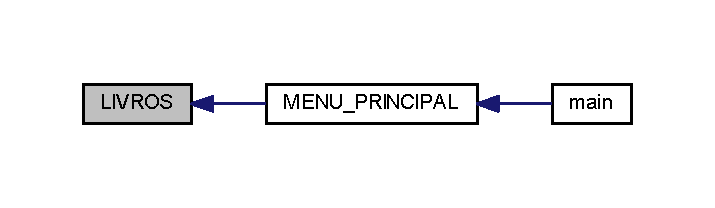
\includegraphics[width=343pt]{1_82__menu_l_i_v_r_o_s_8h_a4e85258e55525e765829f28c4911eb9e_icgraph}
\end{center}
\end{figure}


\hypertarget{1_82__menu_l_i_v_r_o_s_8h_a41a1c98261117fbe5e6f0ebbcec5f9ac}{\index{1.\+2\+\_\+menu\+L\+I\+V\+R\+O\+S.\+h@{1.\+2\+\_\+menu\+L\+I\+V\+R\+O\+S.\+h}!mostrar\+\_\+l@{mostrar\+\_\+l}}
\index{mostrar\+\_\+l@{mostrar\+\_\+l}!1.\+2\+\_\+menu\+L\+I\+V\+R\+O\+S.\+h@{1.\+2\+\_\+menu\+L\+I\+V\+R\+O\+S.\+h}}
\subsubsection[{mostrar\+\_\+l}]{\setlength{\rightskip}{0pt plus 5cm}void mostrar\+\_\+l (
\begin{DoxyParamCaption}
\item[{{\bf livro} $\ast$}]{y}
\end{DoxyParamCaption}
)}}\label{1_82__menu_l_i_v_r_o_s_8h_a41a1c98261117fbe5e6f0ebbcec5f9ac}


Here is the call graph for this function\+:\nopagebreak
\begin{figure}[H]
\begin{center}
\leavevmode
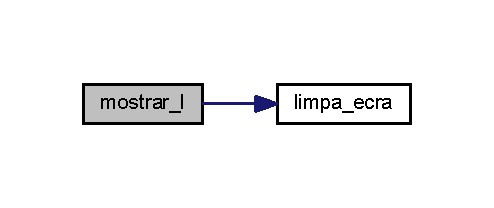
\includegraphics[width=237pt]{1_82__menu_l_i_v_r_o_s_8h_a41a1c98261117fbe5e6f0ebbcec5f9ac_cgraph}
\end{center}
\end{figure}




Here is the caller graph for this function\+:\nopagebreak
\begin{figure}[H]
\begin{center}
\leavevmode
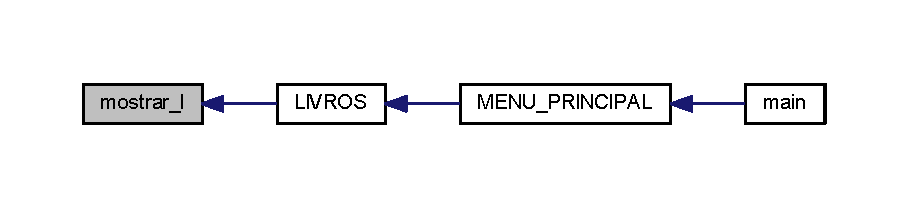
\includegraphics[width=350pt]{1_82__menu_l_i_v_r_o_s_8h_a41a1c98261117fbe5e6f0ebbcec5f9ac_icgraph}
\end{center}
\end{figure}



\hypertarget{1_83__menu_r_e_q_u_i_s_i_c_o_e_s_8h}{\section{source/1.3\+\_\+menu\+R\+E\+Q\+U\+I\+S\+I\+C\+O\+E\+S.h File Reference}
\label{1_83__menu_r_e_q_u_i_s_i_c_o_e_s_8h}\index{source/1.\+3\+\_\+menu\+R\+E\+Q\+U\+I\+S\+I\+C\+O\+E\+S.\+h@{source/1.\+3\+\_\+menu\+R\+E\+Q\+U\+I\+S\+I\+C\+O\+E\+S.\+h}}
}
This graph shows which files directly or indirectly include this file\+:\nopagebreak
\begin{figure}[H]
\begin{center}
\leavevmode
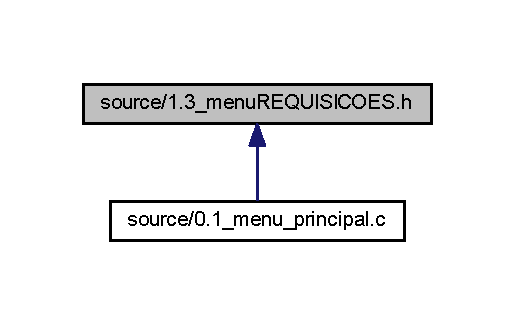
\includegraphics[width=247pt]{1_83__menu_r_e_q_u_i_s_i_c_o_e_s_8h__dep__incl}
\end{center}
\end{figure}
\subsection*{Data Structures}
\begin{DoxyCompactItemize}
\item 
struct \hyperlink{structrequisicao}{requisicao}
\end{DoxyCompactItemize}
\subsection*{Macros}
\begin{DoxyCompactItemize}
\item 
\#define \hyperlink{1_83__menu_r_e_q_u_i_s_i_c_o_e_s_8h_a52037c938e3c1b126c6277da5ca689d0}{M}~100
\end{DoxyCompactItemize}
\subsection*{Functions}
\begin{DoxyCompactItemize}
\item 
void \hyperlink{1_83__menu_r_e_q_u_i_s_i_c_o_e_s_8h_aa92ddaa747cc2f928f3b575451029b81}{ler\+\_\+requisicao} (\hyperlink{structrequisicao}{requisicao} $\ast$z)
\item 
void \hyperlink{1_83__menu_r_e_q_u_i_s_i_c_o_e_s_8h_aa741215de254443a223930c052088a61}{gravar\+\_\+requisicao} (\hyperlink{structrequisicao}{requisicao} $\ast$z)
\item 
void \hyperlink{1_83__menu_r_e_q_u_i_s_i_c_o_e_s_8h_a4694e29d3ee0e145dc50e3501a9f9ed9}{mostrar\+\_\+requisicao} (\hyperlink{structrequisicao}{requisicao} $\ast$z)
\item 
void \hyperlink{1_83__menu_r_e_q_u_i_s_i_c_o_e_s_8h_ade32c575baa0abf818afa59bd549c3a1}{inserir} (\hyperlink{structrequisicao}{requisicao} $\ast$z, \hyperlink{structlivro}{livro} $\ast$y, \hyperlink{structutilizador}{utilizador} $\ast$x)
\item 
int \hyperlink{1_83__menu_r_e_q_u_i_s_i_c_o_e_s_8h_ac632d93f27a41f93bffd78a6ae645d2c}{concluir} (\hyperlink{structrequisicao}{requisicao} $\ast$z)
\item 
void \hyperlink{1_83__menu_r_e_q_u_i_s_i_c_o_e_s_8h_a275551bc2bce83499661b17afc255a7f}{R\+E\+Q\+U\+I\+S\+I\+C\+O\+E\+S} ()
\end{DoxyCompactItemize}


\subsection{Macro Definition Documentation}
\hypertarget{1_83__menu_r_e_q_u_i_s_i_c_o_e_s_8h_a52037c938e3c1b126c6277da5ca689d0}{\index{1.\+3\+\_\+menu\+R\+E\+Q\+U\+I\+S\+I\+C\+O\+E\+S.\+h@{1.\+3\+\_\+menu\+R\+E\+Q\+U\+I\+S\+I\+C\+O\+E\+S.\+h}!M@{M}}
\index{M@{M}!1.\+3\+\_\+menu\+R\+E\+Q\+U\+I\+S\+I\+C\+O\+E\+S.\+h@{1.\+3\+\_\+menu\+R\+E\+Q\+U\+I\+S\+I\+C\+O\+E\+S.\+h}}
\subsubsection[{M}]{\setlength{\rightskip}{0pt plus 5cm}\#define M~100}}\label{1_83__menu_r_e_q_u_i_s_i_c_o_e_s_8h_a52037c938e3c1b126c6277da5ca689d0}


\subsection{Function Documentation}
\hypertarget{1_83__menu_r_e_q_u_i_s_i_c_o_e_s_8h_ac632d93f27a41f93bffd78a6ae645d2c}{\index{1.\+3\+\_\+menu\+R\+E\+Q\+U\+I\+S\+I\+C\+O\+E\+S.\+h@{1.\+3\+\_\+menu\+R\+E\+Q\+U\+I\+S\+I\+C\+O\+E\+S.\+h}!concluir@{concluir}}
\index{concluir@{concluir}!1.\+3\+\_\+menu\+R\+E\+Q\+U\+I\+S\+I\+C\+O\+E\+S.\+h@{1.\+3\+\_\+menu\+R\+E\+Q\+U\+I\+S\+I\+C\+O\+E\+S.\+h}}
\subsubsection[{concluir}]{\setlength{\rightskip}{0pt plus 5cm}int concluir (
\begin{DoxyParamCaption}
\item[{{\bf requisicao} $\ast$}]{z}
\end{DoxyParamCaption}
)}}\label{1_83__menu_r_e_q_u_i_s_i_c_o_e_s_8h_ac632d93f27a41f93bffd78a6ae645d2c}


Here is the caller graph for this function\+:\nopagebreak
\begin{figure}[H]
\begin{center}
\leavevmode
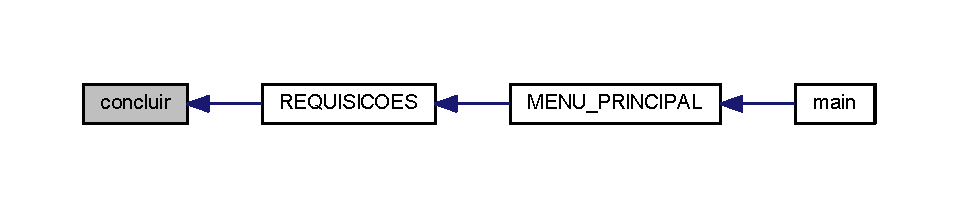
\includegraphics[width=350pt]{1_83__menu_r_e_q_u_i_s_i_c_o_e_s_8h_ac632d93f27a41f93bffd78a6ae645d2c_icgraph}
\end{center}
\end{figure}


\hypertarget{1_83__menu_r_e_q_u_i_s_i_c_o_e_s_8h_aa741215de254443a223930c052088a61}{\index{1.\+3\+\_\+menu\+R\+E\+Q\+U\+I\+S\+I\+C\+O\+E\+S.\+h@{1.\+3\+\_\+menu\+R\+E\+Q\+U\+I\+S\+I\+C\+O\+E\+S.\+h}!gravar\+\_\+requisicao@{gravar\+\_\+requisicao}}
\index{gravar\+\_\+requisicao@{gravar\+\_\+requisicao}!1.\+3\+\_\+menu\+R\+E\+Q\+U\+I\+S\+I\+C\+O\+E\+S.\+h@{1.\+3\+\_\+menu\+R\+E\+Q\+U\+I\+S\+I\+C\+O\+E\+S.\+h}}
\subsubsection[{gravar\+\_\+requisicao}]{\setlength{\rightskip}{0pt plus 5cm}void gravar\+\_\+requisicao (
\begin{DoxyParamCaption}
\item[{{\bf requisicao} $\ast$}]{z}
\end{DoxyParamCaption}
)}}\label{1_83__menu_r_e_q_u_i_s_i_c_o_e_s_8h_aa741215de254443a223930c052088a61}


Here is the caller graph for this function\+:\nopagebreak
\begin{figure}[H]
\begin{center}
\leavevmode
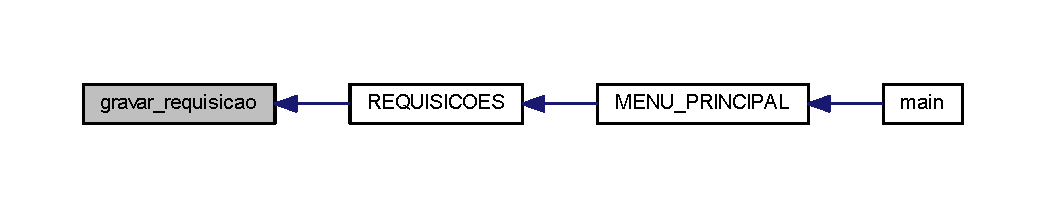
\includegraphics[width=350pt]{1_83__menu_r_e_q_u_i_s_i_c_o_e_s_8h_aa741215de254443a223930c052088a61_icgraph}
\end{center}
\end{figure}


\hypertarget{1_83__menu_r_e_q_u_i_s_i_c_o_e_s_8h_ade32c575baa0abf818afa59bd549c3a1}{\index{1.\+3\+\_\+menu\+R\+E\+Q\+U\+I\+S\+I\+C\+O\+E\+S.\+h@{1.\+3\+\_\+menu\+R\+E\+Q\+U\+I\+S\+I\+C\+O\+E\+S.\+h}!inserir@{inserir}}
\index{inserir@{inserir}!1.\+3\+\_\+menu\+R\+E\+Q\+U\+I\+S\+I\+C\+O\+E\+S.\+h@{1.\+3\+\_\+menu\+R\+E\+Q\+U\+I\+S\+I\+C\+O\+E\+S.\+h}}
\subsubsection[{inserir}]{\setlength{\rightskip}{0pt plus 5cm}void inserir (
\begin{DoxyParamCaption}
\item[{{\bf requisicao} $\ast$}]{z, }
\item[{{\bf livro} $\ast$}]{y, }
\item[{{\bf utilizador} $\ast$}]{x}
\end{DoxyParamCaption}
)}}\label{1_83__menu_r_e_q_u_i_s_i_c_o_e_s_8h_ade32c575baa0abf818afa59bd549c3a1}


Here is the call graph for this function\+:\nopagebreak
\begin{figure}[H]
\begin{center}
\leavevmode
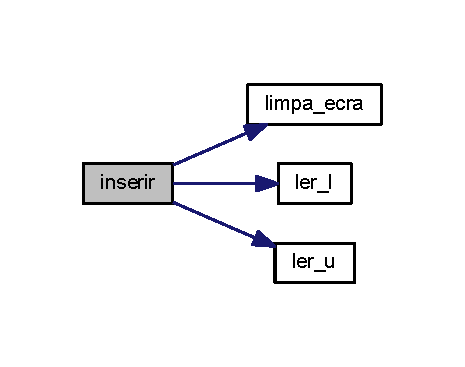
\includegraphics[width=223pt]{1_83__menu_r_e_q_u_i_s_i_c_o_e_s_8h_ade32c575baa0abf818afa59bd549c3a1_cgraph}
\end{center}
\end{figure}




Here is the caller graph for this function\+:\nopagebreak
\begin{figure}[H]
\begin{center}
\leavevmode
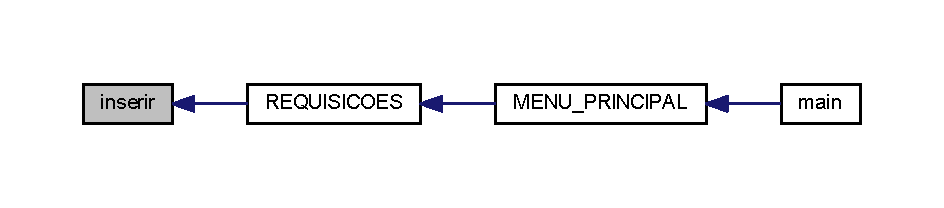
\includegraphics[width=350pt]{1_83__menu_r_e_q_u_i_s_i_c_o_e_s_8h_ade32c575baa0abf818afa59bd549c3a1_icgraph}
\end{center}
\end{figure}


\hypertarget{1_83__menu_r_e_q_u_i_s_i_c_o_e_s_8h_aa92ddaa747cc2f928f3b575451029b81}{\index{1.\+3\+\_\+menu\+R\+E\+Q\+U\+I\+S\+I\+C\+O\+E\+S.\+h@{1.\+3\+\_\+menu\+R\+E\+Q\+U\+I\+S\+I\+C\+O\+E\+S.\+h}!ler\+\_\+requisicao@{ler\+\_\+requisicao}}
\index{ler\+\_\+requisicao@{ler\+\_\+requisicao}!1.\+3\+\_\+menu\+R\+E\+Q\+U\+I\+S\+I\+C\+O\+E\+S.\+h@{1.\+3\+\_\+menu\+R\+E\+Q\+U\+I\+S\+I\+C\+O\+E\+S.\+h}}
\subsubsection[{ler\+\_\+requisicao}]{\setlength{\rightskip}{0pt plus 5cm}void ler\+\_\+requisicao (
\begin{DoxyParamCaption}
\item[{{\bf requisicao} $\ast$}]{z}
\end{DoxyParamCaption}
)}}\label{1_83__menu_r_e_q_u_i_s_i_c_o_e_s_8h_aa92ddaa747cc2f928f3b575451029b81}


Here is the caller graph for this function\+:\nopagebreak
\begin{figure}[H]
\begin{center}
\leavevmode
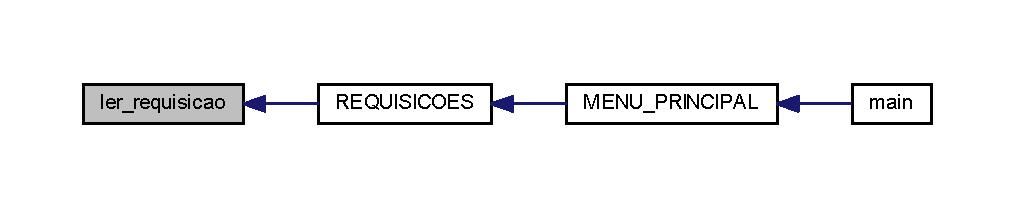
\includegraphics[width=350pt]{1_83__menu_r_e_q_u_i_s_i_c_o_e_s_8h_aa92ddaa747cc2f928f3b575451029b81_icgraph}
\end{center}
\end{figure}


\hypertarget{1_83__menu_r_e_q_u_i_s_i_c_o_e_s_8h_a4694e29d3ee0e145dc50e3501a9f9ed9}{\index{1.\+3\+\_\+menu\+R\+E\+Q\+U\+I\+S\+I\+C\+O\+E\+S.\+h@{1.\+3\+\_\+menu\+R\+E\+Q\+U\+I\+S\+I\+C\+O\+E\+S.\+h}!mostrar\+\_\+requisicao@{mostrar\+\_\+requisicao}}
\index{mostrar\+\_\+requisicao@{mostrar\+\_\+requisicao}!1.\+3\+\_\+menu\+R\+E\+Q\+U\+I\+S\+I\+C\+O\+E\+S.\+h@{1.\+3\+\_\+menu\+R\+E\+Q\+U\+I\+S\+I\+C\+O\+E\+S.\+h}}
\subsubsection[{mostrar\+\_\+requisicao}]{\setlength{\rightskip}{0pt plus 5cm}void mostrar\+\_\+requisicao (
\begin{DoxyParamCaption}
\item[{{\bf requisicao} $\ast$}]{z}
\end{DoxyParamCaption}
)}}\label{1_83__menu_r_e_q_u_i_s_i_c_o_e_s_8h_a4694e29d3ee0e145dc50e3501a9f9ed9}


Here is the caller graph for this function\+:\nopagebreak
\begin{figure}[H]
\begin{center}
\leavevmode
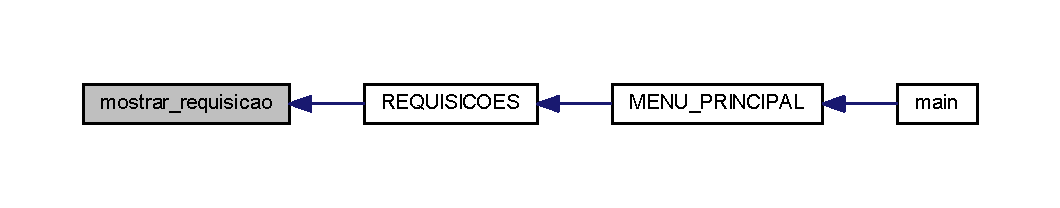
\includegraphics[width=350pt]{1_83__menu_r_e_q_u_i_s_i_c_o_e_s_8h_a4694e29d3ee0e145dc50e3501a9f9ed9_icgraph}
\end{center}
\end{figure}


\hypertarget{1_83__menu_r_e_q_u_i_s_i_c_o_e_s_8h_a275551bc2bce83499661b17afc255a7f}{\index{1.\+3\+\_\+menu\+R\+E\+Q\+U\+I\+S\+I\+C\+O\+E\+S.\+h@{1.\+3\+\_\+menu\+R\+E\+Q\+U\+I\+S\+I\+C\+O\+E\+S.\+h}!R\+E\+Q\+U\+I\+S\+I\+C\+O\+E\+S@{R\+E\+Q\+U\+I\+S\+I\+C\+O\+E\+S}}
\index{R\+E\+Q\+U\+I\+S\+I\+C\+O\+E\+S@{R\+E\+Q\+U\+I\+S\+I\+C\+O\+E\+S}!1.\+3\+\_\+menu\+R\+E\+Q\+U\+I\+S\+I\+C\+O\+E\+S.\+h@{1.\+3\+\_\+menu\+R\+E\+Q\+U\+I\+S\+I\+C\+O\+E\+S.\+h}}
\subsubsection[{R\+E\+Q\+U\+I\+S\+I\+C\+O\+E\+S}]{\setlength{\rightskip}{0pt plus 5cm}void R\+E\+Q\+U\+I\+S\+I\+C\+O\+E\+S (
\begin{DoxyParamCaption}
{}
\end{DoxyParamCaption}
)}}\label{1_83__menu_r_e_q_u_i_s_i_c_o_e_s_8h_a275551bc2bce83499661b17afc255a7f}


Here is the call graph for this function\+:\nopagebreak
\begin{figure}[H]
\begin{center}
\leavevmode
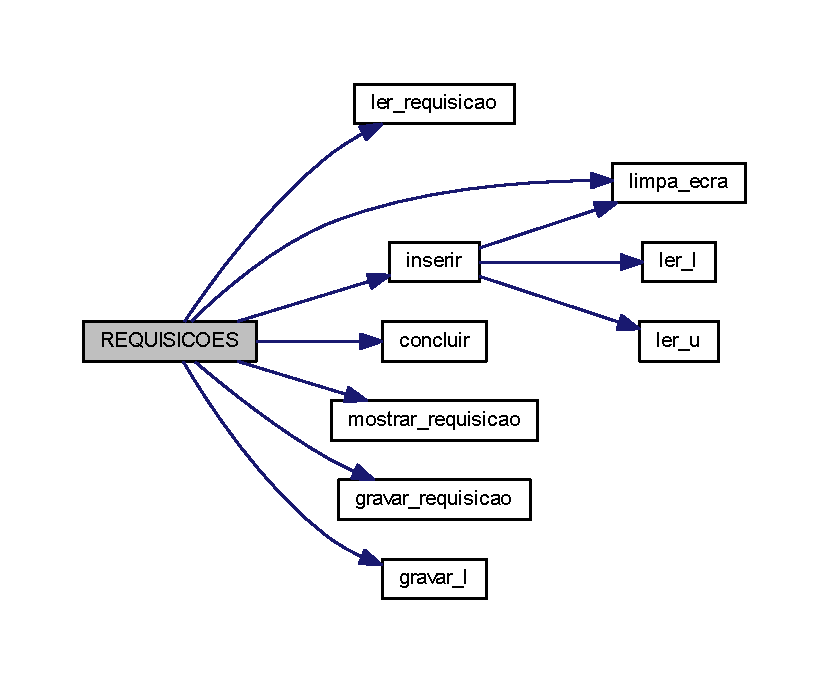
\includegraphics[width=350pt]{1_83__menu_r_e_q_u_i_s_i_c_o_e_s_8h_a275551bc2bce83499661b17afc255a7f_cgraph}
\end{center}
\end{figure}




Here is the caller graph for this function\+:\nopagebreak
\begin{figure}[H]
\begin{center}
\leavevmode
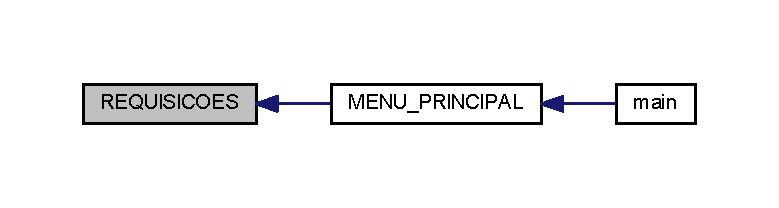
\includegraphics[width=350pt]{1_83__menu_r_e_q_u_i_s_i_c_o_e_s_8h_a275551bc2bce83499661b17afc255a7f_icgraph}
\end{center}
\end{figure}



\hypertarget{1_84__menu_g_e_s_t_a_o_8h}{\section{source/1.4\+\_\+menu\+G\+E\+S\+T\+A\+O.h File Reference}
\label{1_84__menu_g_e_s_t_a_o_8h}\index{source/1.\+4\+\_\+menu\+G\+E\+S\+T\+A\+O.\+h@{source/1.\+4\+\_\+menu\+G\+E\+S\+T\+A\+O.\+h}}
}
\subsection*{Functions}
\begin{DoxyCompactItemize}
\item 
void \hyperlink{1_84__menu_g_e_s_t_a_o_8h_a14effc2d73f1a2f3b49458203ba8af12}{G\+E\+S\+T\+A\+O} ()
\end{DoxyCompactItemize}


\subsection{Function Documentation}
\hypertarget{1_84__menu_g_e_s_t_a_o_8h_a14effc2d73f1a2f3b49458203ba8af12}{\index{1.\+4\+\_\+menu\+G\+E\+S\+T\+A\+O.\+h@{1.\+4\+\_\+menu\+G\+E\+S\+T\+A\+O.\+h}!G\+E\+S\+T\+A\+O@{G\+E\+S\+T\+A\+O}}
\index{G\+E\+S\+T\+A\+O@{G\+E\+S\+T\+A\+O}!1.\+4\+\_\+menu\+G\+E\+S\+T\+A\+O.\+h@{1.\+4\+\_\+menu\+G\+E\+S\+T\+A\+O.\+h}}
\subsubsection[{G\+E\+S\+T\+A\+O}]{\setlength{\rightskip}{0pt plus 5cm}void G\+E\+S\+T\+A\+O (
\begin{DoxyParamCaption}
{}
\end{DoxyParamCaption}
)}}\label{1_84__menu_g_e_s_t_a_o_8h_a14effc2d73f1a2f3b49458203ba8af12}

\hypertarget{_projeto1__private_8h}{\section{source/\+Projeto1\+\_\+private.h File Reference}
\label{_projeto1__private_8h}\index{source/\+Projeto1\+\_\+private.\+h@{source/\+Projeto1\+\_\+private.\+h}}
}
\subsection*{Macros}
\begin{DoxyCompactItemize}
\item 
\#define \hyperlink{_projeto1__private_8h_aec977eff8d77d9c22f46665015a6f239}{V\+E\+R\+\_\+\+S\+T\+R\+I\+N\+G}~\char`\"{}1.\+0.\+1.\+2\char`\"{}
\item 
\#define \hyperlink{_projeto1__private_8h_ae9b0873c1004a01651f733d556db118c}{V\+E\+R\+\_\+\+M\+A\+J\+O\+R}~1
\item 
\#define \hyperlink{_projeto1__private_8h_ad78650efa42849c5f86d372f11f26403}{V\+E\+R\+\_\+\+M\+I\+N\+O\+R}~0
\item 
\#define \hyperlink{_projeto1__private_8h_a3addb24971814c8e78cf3872dd643a48}{V\+E\+R\+\_\+\+R\+E\+L\+E\+A\+S\+E}~1
\item 
\#define \hyperlink{_projeto1__private_8h_a7ce3a6824adeecbb4481086e2ba00fb8}{V\+E\+R\+\_\+\+B\+U\+I\+L\+D}~2
\item 
\#define \hyperlink{_projeto1__private_8h_a9c76a8ad5fd75187ad154a79d392dfc2}{C\+O\+M\+P\+A\+N\+Y\+\_\+\+N\+A\+M\+E}~\char`\"{}tic\char`\"{}
\item 
\#define \hyperlink{_projeto1__private_8h_a78550c98b8cfa286587b618347dc3011}{F\+I\+L\+E\+\_\+\+V\+E\+R\+S\+I\+O\+N}~\char`\"{}1.\+0.\+1.\+2\char`\"{}
\item 
\#define \hyperlink{_projeto1__private_8h_a01192f4cf039acedc3ac603f80f59184}{F\+I\+L\+E\+\_\+\+D\+E\+S\+C\+R\+I\+P\+T\+I\+O\+N}~\char`\"{}Developed using the Dev-\/C++ I\+D\+E\char`\"{}
\item 
\#define \hyperlink{_projeto1__private_8h_a8a8c7bc542435504233c139db8466fa5}{I\+N\+T\+E\+R\+N\+A\+L\+\_\+\+N\+A\+M\+E}~\char`\"{}\char`\"{}
\item 
\#define \hyperlink{_projeto1__private_8h_a8b95afde376bc69dc26a267786125074}{L\+E\+G\+A\+L\+\_\+\+C\+O\+P\+Y\+R\+I\+G\+H\+T}~\char`\"{}tic\char`\"{}
\item 
\#define \hyperlink{_projeto1__private_8h_ae4fa88b4630b8cd07bc0bd4bd90ca816}{L\+E\+G\+A\+L\+\_\+\+T\+R\+A\+D\+E\+M\+A\+R\+K\+S}~\char`\"{}tic\char`\"{}
\item 
\#define \hyperlink{_projeto1__private_8h_a60d025b4ac9be9b1a924be9d15b2d4a3}{O\+R\+I\+G\+I\+N\+A\+L\+\_\+\+F\+I\+L\+E\+N\+A\+M\+E}~\char`\"{}\char`\"{}
\item 
\#define \hyperlink{_projeto1__private_8h_a2fd81ded1b6a151f629441182c358d5b}{P\+R\+O\+D\+U\+C\+T\+\_\+\+N\+A\+M\+E}~\char`\"{}Biblioteca universal\char`\"{}
\item 
\#define \hyperlink{_projeto1__private_8h_a0ba1a85361118228096108c7d425f84b}{P\+R\+O\+D\+U\+C\+T\+\_\+\+V\+E\+R\+S\+I\+O\+N}~\char`\"{}1.\+0.\+1.\+2\char`\"{}
\end{DoxyCompactItemize}


\subsection{Macro Definition Documentation}
\hypertarget{_projeto1__private_8h_a9c76a8ad5fd75187ad154a79d392dfc2}{\index{Projeto1\+\_\+private.\+h@{Projeto1\+\_\+private.\+h}!C\+O\+M\+P\+A\+N\+Y\+\_\+\+N\+A\+M\+E@{C\+O\+M\+P\+A\+N\+Y\+\_\+\+N\+A\+M\+E}}
\index{C\+O\+M\+P\+A\+N\+Y\+\_\+\+N\+A\+M\+E@{C\+O\+M\+P\+A\+N\+Y\+\_\+\+N\+A\+M\+E}!Projeto1\+\_\+private.\+h@{Projeto1\+\_\+private.\+h}}
\subsubsection[{C\+O\+M\+P\+A\+N\+Y\+\_\+\+N\+A\+M\+E}]{\setlength{\rightskip}{0pt plus 5cm}\#define C\+O\+M\+P\+A\+N\+Y\+\_\+\+N\+A\+M\+E~\char`\"{}tic\char`\"{}}}\label{_projeto1__private_8h_a9c76a8ad5fd75187ad154a79d392dfc2}
\hypertarget{_projeto1__private_8h_a01192f4cf039acedc3ac603f80f59184}{\index{Projeto1\+\_\+private.\+h@{Projeto1\+\_\+private.\+h}!F\+I\+L\+E\+\_\+\+D\+E\+S\+C\+R\+I\+P\+T\+I\+O\+N@{F\+I\+L\+E\+\_\+\+D\+E\+S\+C\+R\+I\+P\+T\+I\+O\+N}}
\index{F\+I\+L\+E\+\_\+\+D\+E\+S\+C\+R\+I\+P\+T\+I\+O\+N@{F\+I\+L\+E\+\_\+\+D\+E\+S\+C\+R\+I\+P\+T\+I\+O\+N}!Projeto1\+\_\+private.\+h@{Projeto1\+\_\+private.\+h}}
\subsubsection[{F\+I\+L\+E\+\_\+\+D\+E\+S\+C\+R\+I\+P\+T\+I\+O\+N}]{\setlength{\rightskip}{0pt plus 5cm}\#define F\+I\+L\+E\+\_\+\+D\+E\+S\+C\+R\+I\+P\+T\+I\+O\+N~\char`\"{}Developed using the Dev-\/C++ I\+D\+E\char`\"{}}}\label{_projeto1__private_8h_a01192f4cf039acedc3ac603f80f59184}
\hypertarget{_projeto1__private_8h_a78550c98b8cfa286587b618347dc3011}{\index{Projeto1\+\_\+private.\+h@{Projeto1\+\_\+private.\+h}!F\+I\+L\+E\+\_\+\+V\+E\+R\+S\+I\+O\+N@{F\+I\+L\+E\+\_\+\+V\+E\+R\+S\+I\+O\+N}}
\index{F\+I\+L\+E\+\_\+\+V\+E\+R\+S\+I\+O\+N@{F\+I\+L\+E\+\_\+\+V\+E\+R\+S\+I\+O\+N}!Projeto1\+\_\+private.\+h@{Projeto1\+\_\+private.\+h}}
\subsubsection[{F\+I\+L\+E\+\_\+\+V\+E\+R\+S\+I\+O\+N}]{\setlength{\rightskip}{0pt plus 5cm}\#define F\+I\+L\+E\+\_\+\+V\+E\+R\+S\+I\+O\+N~\char`\"{}1.\+0.\+1.\+2\char`\"{}}}\label{_projeto1__private_8h_a78550c98b8cfa286587b618347dc3011}
\hypertarget{_projeto1__private_8h_a8a8c7bc542435504233c139db8466fa5}{\index{Projeto1\+\_\+private.\+h@{Projeto1\+\_\+private.\+h}!I\+N\+T\+E\+R\+N\+A\+L\+\_\+\+N\+A\+M\+E@{I\+N\+T\+E\+R\+N\+A\+L\+\_\+\+N\+A\+M\+E}}
\index{I\+N\+T\+E\+R\+N\+A\+L\+\_\+\+N\+A\+M\+E@{I\+N\+T\+E\+R\+N\+A\+L\+\_\+\+N\+A\+M\+E}!Projeto1\+\_\+private.\+h@{Projeto1\+\_\+private.\+h}}
\subsubsection[{I\+N\+T\+E\+R\+N\+A\+L\+\_\+\+N\+A\+M\+E}]{\setlength{\rightskip}{0pt plus 5cm}\#define I\+N\+T\+E\+R\+N\+A\+L\+\_\+\+N\+A\+M\+E~\char`\"{}\char`\"{}}}\label{_projeto1__private_8h_a8a8c7bc542435504233c139db8466fa5}
\hypertarget{_projeto1__private_8h_a8b95afde376bc69dc26a267786125074}{\index{Projeto1\+\_\+private.\+h@{Projeto1\+\_\+private.\+h}!L\+E\+G\+A\+L\+\_\+\+C\+O\+P\+Y\+R\+I\+G\+H\+T@{L\+E\+G\+A\+L\+\_\+\+C\+O\+P\+Y\+R\+I\+G\+H\+T}}
\index{L\+E\+G\+A\+L\+\_\+\+C\+O\+P\+Y\+R\+I\+G\+H\+T@{L\+E\+G\+A\+L\+\_\+\+C\+O\+P\+Y\+R\+I\+G\+H\+T}!Projeto1\+\_\+private.\+h@{Projeto1\+\_\+private.\+h}}
\subsubsection[{L\+E\+G\+A\+L\+\_\+\+C\+O\+P\+Y\+R\+I\+G\+H\+T}]{\setlength{\rightskip}{0pt plus 5cm}\#define L\+E\+G\+A\+L\+\_\+\+C\+O\+P\+Y\+R\+I\+G\+H\+T~\char`\"{}tic\char`\"{}}}\label{_projeto1__private_8h_a8b95afde376bc69dc26a267786125074}
\hypertarget{_projeto1__private_8h_ae4fa88b4630b8cd07bc0bd4bd90ca816}{\index{Projeto1\+\_\+private.\+h@{Projeto1\+\_\+private.\+h}!L\+E\+G\+A\+L\+\_\+\+T\+R\+A\+D\+E\+M\+A\+R\+K\+S@{L\+E\+G\+A\+L\+\_\+\+T\+R\+A\+D\+E\+M\+A\+R\+K\+S}}
\index{L\+E\+G\+A\+L\+\_\+\+T\+R\+A\+D\+E\+M\+A\+R\+K\+S@{L\+E\+G\+A\+L\+\_\+\+T\+R\+A\+D\+E\+M\+A\+R\+K\+S}!Projeto1\+\_\+private.\+h@{Projeto1\+\_\+private.\+h}}
\subsubsection[{L\+E\+G\+A\+L\+\_\+\+T\+R\+A\+D\+E\+M\+A\+R\+K\+S}]{\setlength{\rightskip}{0pt plus 5cm}\#define L\+E\+G\+A\+L\+\_\+\+T\+R\+A\+D\+E\+M\+A\+R\+K\+S~\char`\"{}tic\char`\"{}}}\label{_projeto1__private_8h_ae4fa88b4630b8cd07bc0bd4bd90ca816}
\hypertarget{_projeto1__private_8h_a60d025b4ac9be9b1a924be9d15b2d4a3}{\index{Projeto1\+\_\+private.\+h@{Projeto1\+\_\+private.\+h}!O\+R\+I\+G\+I\+N\+A\+L\+\_\+\+F\+I\+L\+E\+N\+A\+M\+E@{O\+R\+I\+G\+I\+N\+A\+L\+\_\+\+F\+I\+L\+E\+N\+A\+M\+E}}
\index{O\+R\+I\+G\+I\+N\+A\+L\+\_\+\+F\+I\+L\+E\+N\+A\+M\+E@{O\+R\+I\+G\+I\+N\+A\+L\+\_\+\+F\+I\+L\+E\+N\+A\+M\+E}!Projeto1\+\_\+private.\+h@{Projeto1\+\_\+private.\+h}}
\subsubsection[{O\+R\+I\+G\+I\+N\+A\+L\+\_\+\+F\+I\+L\+E\+N\+A\+M\+E}]{\setlength{\rightskip}{0pt plus 5cm}\#define O\+R\+I\+G\+I\+N\+A\+L\+\_\+\+F\+I\+L\+E\+N\+A\+M\+E~\char`\"{}\char`\"{}}}\label{_projeto1__private_8h_a60d025b4ac9be9b1a924be9d15b2d4a3}
\hypertarget{_projeto1__private_8h_a2fd81ded1b6a151f629441182c358d5b}{\index{Projeto1\+\_\+private.\+h@{Projeto1\+\_\+private.\+h}!P\+R\+O\+D\+U\+C\+T\+\_\+\+N\+A\+M\+E@{P\+R\+O\+D\+U\+C\+T\+\_\+\+N\+A\+M\+E}}
\index{P\+R\+O\+D\+U\+C\+T\+\_\+\+N\+A\+M\+E@{P\+R\+O\+D\+U\+C\+T\+\_\+\+N\+A\+M\+E}!Projeto1\+\_\+private.\+h@{Projeto1\+\_\+private.\+h}}
\subsubsection[{P\+R\+O\+D\+U\+C\+T\+\_\+\+N\+A\+M\+E}]{\setlength{\rightskip}{0pt plus 5cm}\#define P\+R\+O\+D\+U\+C\+T\+\_\+\+N\+A\+M\+E~\char`\"{}Biblioteca universal\char`\"{}}}\label{_projeto1__private_8h_a2fd81ded1b6a151f629441182c358d5b}
\hypertarget{_projeto1__private_8h_a0ba1a85361118228096108c7d425f84b}{\index{Projeto1\+\_\+private.\+h@{Projeto1\+\_\+private.\+h}!P\+R\+O\+D\+U\+C\+T\+\_\+\+V\+E\+R\+S\+I\+O\+N@{P\+R\+O\+D\+U\+C\+T\+\_\+\+V\+E\+R\+S\+I\+O\+N}}
\index{P\+R\+O\+D\+U\+C\+T\+\_\+\+V\+E\+R\+S\+I\+O\+N@{P\+R\+O\+D\+U\+C\+T\+\_\+\+V\+E\+R\+S\+I\+O\+N}!Projeto1\+\_\+private.\+h@{Projeto1\+\_\+private.\+h}}
\subsubsection[{P\+R\+O\+D\+U\+C\+T\+\_\+\+V\+E\+R\+S\+I\+O\+N}]{\setlength{\rightskip}{0pt plus 5cm}\#define P\+R\+O\+D\+U\+C\+T\+\_\+\+V\+E\+R\+S\+I\+O\+N~\char`\"{}1.\+0.\+1.\+2\char`\"{}}}\label{_projeto1__private_8h_a0ba1a85361118228096108c7d425f84b}
\hypertarget{_projeto1__private_8h_a7ce3a6824adeecbb4481086e2ba00fb8}{\index{Projeto1\+\_\+private.\+h@{Projeto1\+\_\+private.\+h}!V\+E\+R\+\_\+\+B\+U\+I\+L\+D@{V\+E\+R\+\_\+\+B\+U\+I\+L\+D}}
\index{V\+E\+R\+\_\+\+B\+U\+I\+L\+D@{V\+E\+R\+\_\+\+B\+U\+I\+L\+D}!Projeto1\+\_\+private.\+h@{Projeto1\+\_\+private.\+h}}
\subsubsection[{V\+E\+R\+\_\+\+B\+U\+I\+L\+D}]{\setlength{\rightskip}{0pt plus 5cm}\#define V\+E\+R\+\_\+\+B\+U\+I\+L\+D~2}}\label{_projeto1__private_8h_a7ce3a6824adeecbb4481086e2ba00fb8}
\hypertarget{_projeto1__private_8h_ae9b0873c1004a01651f733d556db118c}{\index{Projeto1\+\_\+private.\+h@{Projeto1\+\_\+private.\+h}!V\+E\+R\+\_\+\+M\+A\+J\+O\+R@{V\+E\+R\+\_\+\+M\+A\+J\+O\+R}}
\index{V\+E\+R\+\_\+\+M\+A\+J\+O\+R@{V\+E\+R\+\_\+\+M\+A\+J\+O\+R}!Projeto1\+\_\+private.\+h@{Projeto1\+\_\+private.\+h}}
\subsubsection[{V\+E\+R\+\_\+\+M\+A\+J\+O\+R}]{\setlength{\rightskip}{0pt plus 5cm}\#define V\+E\+R\+\_\+\+M\+A\+J\+O\+R~1}}\label{_projeto1__private_8h_ae9b0873c1004a01651f733d556db118c}
\hypertarget{_projeto1__private_8h_ad78650efa42849c5f86d372f11f26403}{\index{Projeto1\+\_\+private.\+h@{Projeto1\+\_\+private.\+h}!V\+E\+R\+\_\+\+M\+I\+N\+O\+R@{V\+E\+R\+\_\+\+M\+I\+N\+O\+R}}
\index{V\+E\+R\+\_\+\+M\+I\+N\+O\+R@{V\+E\+R\+\_\+\+M\+I\+N\+O\+R}!Projeto1\+\_\+private.\+h@{Projeto1\+\_\+private.\+h}}
\subsubsection[{V\+E\+R\+\_\+\+M\+I\+N\+O\+R}]{\setlength{\rightskip}{0pt plus 5cm}\#define V\+E\+R\+\_\+\+M\+I\+N\+O\+R~0}}\label{_projeto1__private_8h_ad78650efa42849c5f86d372f11f26403}
\hypertarget{_projeto1__private_8h_a3addb24971814c8e78cf3872dd643a48}{\index{Projeto1\+\_\+private.\+h@{Projeto1\+\_\+private.\+h}!V\+E\+R\+\_\+\+R\+E\+L\+E\+A\+S\+E@{V\+E\+R\+\_\+\+R\+E\+L\+E\+A\+S\+E}}
\index{V\+E\+R\+\_\+\+R\+E\+L\+E\+A\+S\+E@{V\+E\+R\+\_\+\+R\+E\+L\+E\+A\+S\+E}!Projeto1\+\_\+private.\+h@{Projeto1\+\_\+private.\+h}}
\subsubsection[{V\+E\+R\+\_\+\+R\+E\+L\+E\+A\+S\+E}]{\setlength{\rightskip}{0pt plus 5cm}\#define V\+E\+R\+\_\+\+R\+E\+L\+E\+A\+S\+E~1}}\label{_projeto1__private_8h_a3addb24971814c8e78cf3872dd643a48}
\hypertarget{_projeto1__private_8h_aec977eff8d77d9c22f46665015a6f239}{\index{Projeto1\+\_\+private.\+h@{Projeto1\+\_\+private.\+h}!V\+E\+R\+\_\+\+S\+T\+R\+I\+N\+G@{V\+E\+R\+\_\+\+S\+T\+R\+I\+N\+G}}
\index{V\+E\+R\+\_\+\+S\+T\+R\+I\+N\+G@{V\+E\+R\+\_\+\+S\+T\+R\+I\+N\+G}!Projeto1\+\_\+private.\+h@{Projeto1\+\_\+private.\+h}}
\subsubsection[{V\+E\+R\+\_\+\+S\+T\+R\+I\+N\+G}]{\setlength{\rightskip}{0pt plus 5cm}\#define V\+E\+R\+\_\+\+S\+T\+R\+I\+N\+G~\char`\"{}1.\+0.\+1.\+2\char`\"{}}}\label{_projeto1__private_8h_aec977eff8d77d9c22f46665015a6f239}

\hypertarget{relogio_8h}{\section{source/relogio.h File Reference}
\label{relogio_8h}\index{source/relogio.\+h@{source/relogio.\+h}}
}
This graph shows which files directly or indirectly include this file\+:\nopagebreak
\begin{figure}[H]
\begin{center}
\leavevmode
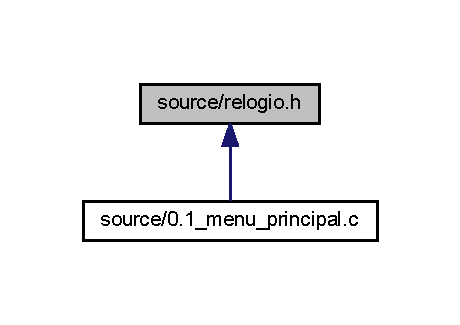
\includegraphics[width=221pt]{relogio_8h__dep__incl}
\end{center}
\end{figure}
\subsection*{Functions}
\begin{DoxyCompactItemize}
\item 
int \hyperlink{relogio_8h_ad2c584e6472d5514c2fa94aea1697bb7}{t} (void)
\end{DoxyCompactItemize}


\subsection{Function Documentation}
\hypertarget{relogio_8h_ad2c584e6472d5514c2fa94aea1697bb7}{\index{relogio.\+h@{relogio.\+h}!t@{t}}
\index{t@{t}!relogio.\+h@{relogio.\+h}}
\subsubsection[{t}]{\setlength{\rightskip}{0pt plus 5cm}int t (
\begin{DoxyParamCaption}
\item[{void}]{}
\end{DoxyParamCaption}
)}}\label{relogio_8h_ad2c584e6472d5514c2fa94aea1697bb7}


Here is the caller graph for this function\+:\nopagebreak
\begin{figure}[H]
\begin{center}
\leavevmode
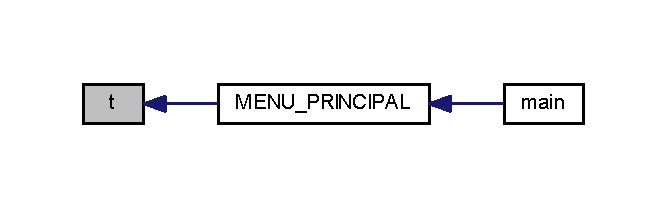
\includegraphics[width=320pt]{relogio_8h_ad2c584e6472d5514c2fa94aea1697bb7_icgraph}
\end{center}
\end{figure}



%--- End generated contents ---

% Index
\newpage
\phantomsection
\addcontentsline{toc}{chapter}{Index}
\printindex

\end{document}
